
    




    
\documentclass[11pt]{article}

    
    \usepackage[breakable]{tcolorbox}
    \tcbset{nobeforeafter} % prevents tcolorboxes being placing in paragraphs
    \usepackage{float}
    \floatplacement{figure}{H} % forces figures to be placed at the correct location
    
    \usepackage[T1]{fontenc}
    % Nicer default font (+ math font) than Computer Modern for most use cases
    \usepackage{mathpazo}

    % Basic figure setup, for now with no caption control since it's done
    % automatically by Pandoc (which extracts ![](path) syntax from Markdown).
    \usepackage{graphicx}
    % We will generate all images so they have a width \maxwidth. This means
    % that they will get their normal width if they fit onto the page, but
    % are scaled down if they would overflow the margins.
    \makeatletter
    \def\maxwidth{\ifdim\Gin@nat@width>\linewidth\linewidth
    \else\Gin@nat@width\fi}
    \makeatother
    \let\Oldincludegraphics\includegraphics
    % Set max figure width to be 80% of text width, for now hardcoded.
    \renewcommand{\includegraphics}[1]{\Oldincludegraphics[width=.8\maxwidth]{#1}}
    % Ensure that by default, figures have no caption (until we provide a
    % proper Figure object with a Caption API and a way to capture that
    % in the conversion process - todo).
    \usepackage{caption}
    \DeclareCaptionLabelFormat{nolabel}{}
    \captionsetup{labelformat=nolabel}

    \usepackage{adjustbox} % Used to constrain images to a maximum size 
    \usepackage{xcolor} % Allow colors to be defined
    \usepackage{enumerate} % Needed for markdown enumerations to work
    \usepackage{geometry} % Used to adjust the document margins
    \usepackage{amsmath} % Equations
    \usepackage{amssymb} % Equations
    \usepackage{textcomp} % defines textquotesingle
    % Hack from http://tex.stackexchange.com/a/47451/13684:
    \AtBeginDocument{%
        \def\PYZsq{\textquotesingle}% Upright quotes in Pygmentized code
    }
    \usepackage{upquote} % Upright quotes for verbatim code
    \usepackage{eurosym} % defines \euro
    \usepackage[mathletters]{ucs} % Extended unicode (utf-8) support
    %\usepackage[utf8x]{inputenc} % Allow utf-8 characters in the tex document
	\usepackage[utf8]{inputenc} % Allow utf-8 characters in the tex document	\usepackage[spanish]{babel}
    \usepackage{fancyvrb} % verbatim replacement that allows latex
    \usepackage{grffile} % extends the file name processing of package graphics 
                         % to support a larger range 
    % The hyperref package gives us a pdf with properly built
    % internal navigation ('pdf bookmarks' for the table of contents,
    % internal cross-reference links, web links for URLs, etc.)
    \usepackage{hyperref}
    \usepackage{longtable} % longtable support required by pandoc >1.10
    \usepackage{booktabs}  % table support for pandoc > 1.12.2
    \usepackage[inline]{enumitem} % IRkernel/repr support (it uses the enumerate* environment)
    \usepackage[normalem]{ulem} % ulem is needed to support strikethroughs (\sout)
                                % normalem makes italics be italics, not underlines
    \usepackage{mathrsfs}
    

    
    % Colors for the hyperref package
    \definecolor{urlcolor}{rgb}{0,.145,.698}
    \definecolor{linkcolor}{rgb}{.71,0.21,0.01}
    \definecolor{citecolor}{rgb}{.12,.54,.11}

    % ANSI colors
    \definecolor{ansi-black}{HTML}{3E424D}
    \definecolor{ansi-black-intense}{HTML}{282C36}
    \definecolor{ansi-red}{HTML}{E75C58}
    \definecolor{ansi-red-intense}{HTML}{B22B31}
    \definecolor{ansi-green}{HTML}{00A250}
    \definecolor{ansi-green-intense}{HTML}{007427}
    \definecolor{ansi-yellow}{HTML}{DDB62B}
    \definecolor{ansi-yellow-intense}{HTML}{B27D12}
    \definecolor{ansi-blue}{HTML}{208FFB}
    \definecolor{ansi-blue-intense}{HTML}{0065CA}
    \definecolor{ansi-magenta}{HTML}{D160C4}
    \definecolor{ansi-magenta-intense}{HTML}{A03196}
    \definecolor{ansi-cyan}{HTML}{60C6C8}
    \definecolor{ansi-cyan-intense}{HTML}{258F8F}
    \definecolor{ansi-white}{HTML}{C5C1B4}
    \definecolor{ansi-white-intense}{HTML}{A1A6B2}
    \definecolor{ansi-default-inverse-fg}{HTML}{FFFFFF}
    \definecolor{ansi-default-inverse-bg}{HTML}{000000}

    % commands and environments needed by pandoc snippets
    % extracted from the output of `pandoc -s`
    \providecommand{\tightlist}{%
      \setlength{\itemsep}{0pt}\setlength{\parskip}{0pt}}
    \DefineVerbatimEnvironment{Highlighting}{Verbatim}{commandchars=\\\{\}}
    % Add ',fontsize=\small' for more characters per line
    \newenvironment{Shaded}{}{}
    \newcommand{\KeywordTok}[1]{\textcolor[rgb]{0.00,0.44,0.13}{\textbf{{#1}}}}
    \newcommand{\DataTypeTok}[1]{\textcolor[rgb]{0.56,0.13,0.00}{{#1}}}
    \newcommand{\DecValTok}[1]{\textcolor[rgb]{0.25,0.63,0.44}{{#1}}}
    \newcommand{\BaseNTok}[1]{\textcolor[rgb]{0.25,0.63,0.44}{{#1}}}
    \newcommand{\FloatTok}[1]{\textcolor[rgb]{0.25,0.63,0.44}{{#1}}}
    \newcommand{\CharTok}[1]{\textcolor[rgb]{0.25,0.44,0.63}{{#1}}}
    \newcommand{\StringTok}[1]{\textcolor[rgb]{0.25,0.44,0.63}{{#1}}}
    \newcommand{\CommentTok}[1]{\textcolor[rgb]{0.38,0.63,0.69}{\textit{{#1}}}}
    \newcommand{\OtherTok}[1]{\textcolor[rgb]{0.00,0.44,0.13}{{#1}}}
    \newcommand{\AlertTok}[1]{\textcolor[rgb]{1.00,0.00,0.00}{\textbf{{#1}}}}
    \newcommand{\FunctionTok}[1]{\textcolor[rgb]{0.02,0.16,0.49}{{#1}}}
    \newcommand{\RegionMarkerTok}[1]{{#1}}
    \newcommand{\ErrorTok}[1]{\textcolor[rgb]{1.00,0.00,0.00}{\textbf{{#1}}}}
    \newcommand{\NormalTok}[1]{{#1}}
    
    % Additional commands for more recent versions of Pandoc
    \newcommand{\ConstantTok}[1]{\textcolor[rgb]{0.53,0.00,0.00}{{#1}}}
    \newcommand{\SpecialCharTok}[1]{\textcolor[rgb]{0.25,0.44,0.63}{{#1}}}
    \newcommand{\VerbatimStringTok}[1]{\textcolor[rgb]{0.25,0.44,0.63}{{#1}}}
    \newcommand{\SpecialStringTok}[1]{\textcolor[rgb]{0.73,0.40,0.53}{{#1}}}
    \newcommand{\ImportTok}[1]{{#1}}
    \newcommand{\DocumentationTok}[1]{\textcolor[rgb]{0.73,0.13,0.13}{\textit{{#1}}}}
    \newcommand{\AnnotationTok}[1]{\textcolor[rgb]{0.38,0.63,0.69}{\textbf{\textit{{#1}}}}}
    \newcommand{\CommentVarTok}[1]{\textcolor[rgb]{0.38,0.63,0.69}{\textbf{\textit{{#1}}}}}
    \newcommand{\VariableTok}[1]{\textcolor[rgb]{0.10,0.09,0.49}{{#1}}}
    \newcommand{\ControlFlowTok}[1]{\textcolor[rgb]{0.00,0.44,0.13}{\textbf{{#1}}}}
    \newcommand{\OperatorTok}[1]{\textcolor[rgb]{0.40,0.40,0.40}{{#1}}}
    \newcommand{\BuiltInTok}[1]{{#1}}
    \newcommand{\ExtensionTok}[1]{{#1}}
    \newcommand{\PreprocessorTok}[1]{\textcolor[rgb]{0.74,0.48,0.00}{{#1}}}
    \newcommand{\AttributeTok}[1]{\textcolor[rgb]{0.49,0.56,0.16}{{#1}}}
    \newcommand{\InformationTok}[1]{\textcolor[rgb]{0.38,0.63,0.69}{\textbf{\textit{{#1}}}}}
    \newcommand{\WarningTok}[1]{\textcolor[rgb]{0.38,0.63,0.69}{\textbf{\textit{{#1}}}}}
    
    
    % Define a nice break command that doesn't care if a line doesn't already
    % exist.
    \def\br{\hspace*{\fill} \\* }
    % Math Jax compatibility definitions
    \def\gt{>}
    \def\lt{<}
    \let\Oldtex\TeX
    \let\Oldlatex\LaTeX
    \renewcommand{\TeX}{\textrm{\Oldtex}}
    \renewcommand{\LaTeX}{\textrm{\Oldlatex}}
    % Document parameters
    % Document title
    \title{TPE-95874}
    
    
    
    
    
% Pygments definitions
\makeatletter
\def\PY@reset{\let\PY@it=\relax \let\PY@bf=\relax%
    \let\PY@ul=\relax \let\PY@tc=\relax%
    \let\PY@bc=\relax \let\PY@ff=\relax}
\def\PY@tok#1{\csname PY@tok@#1\endcsname}
\def\PY@toks#1+{\ifx\relax#1\empty\else%
    \PY@tok{#1}\expandafter\PY@toks\fi}
\def\PY@do#1{\PY@bc{\PY@tc{\PY@ul{%
    \PY@it{\PY@bf{\PY@ff{#1}}}}}}}
\def\PY#1#2{\PY@reset\PY@toks#1+\relax+\PY@do{#2}}

\expandafter\def\csname PY@tok@w\endcsname{\def\PY@tc##1{\textcolor[rgb]{0.73,0.73,0.73}{##1}}}
\expandafter\def\csname PY@tok@c\endcsname{\let\PY@it=\textit\def\PY@tc##1{\textcolor[rgb]{0.25,0.50,0.50}{##1}}}
\expandafter\def\csname PY@tok@cp\endcsname{\def\PY@tc##1{\textcolor[rgb]{0.74,0.48,0.00}{##1}}}
\expandafter\def\csname PY@tok@k\endcsname{\let\PY@bf=\textbf\def\PY@tc##1{\textcolor[rgb]{0.00,0.50,0.00}{##1}}}
\expandafter\def\csname PY@tok@kp\endcsname{\def\PY@tc##1{\textcolor[rgb]{0.00,0.50,0.00}{##1}}}
\expandafter\def\csname PY@tok@kt\endcsname{\def\PY@tc##1{\textcolor[rgb]{0.69,0.00,0.25}{##1}}}
\expandafter\def\csname PY@tok@o\endcsname{\def\PY@tc##1{\textcolor[rgb]{0.40,0.40,0.40}{##1}}}
\expandafter\def\csname PY@tok@ow\endcsname{\let\PY@bf=\textbf\def\PY@tc##1{\textcolor[rgb]{0.67,0.13,1.00}{##1}}}
\expandafter\def\csname PY@tok@nb\endcsname{\def\PY@tc##1{\textcolor[rgb]{0.00,0.50,0.00}{##1}}}
\expandafter\def\csname PY@tok@nf\endcsname{\def\PY@tc##1{\textcolor[rgb]{0.00,0.00,1.00}{##1}}}
\expandafter\def\csname PY@tok@nc\endcsname{\let\PY@bf=\textbf\def\PY@tc##1{\textcolor[rgb]{0.00,0.00,1.00}{##1}}}
\expandafter\def\csname PY@tok@nn\endcsname{\let\PY@bf=\textbf\def\PY@tc##1{\textcolor[rgb]{0.00,0.00,1.00}{##1}}}
\expandafter\def\csname PY@tok@ne\endcsname{\let\PY@bf=\textbf\def\PY@tc##1{\textcolor[rgb]{0.82,0.25,0.23}{##1}}}
\expandafter\def\csname PY@tok@nv\endcsname{\def\PY@tc##1{\textcolor[rgb]{0.10,0.09,0.49}{##1}}}
\expandafter\def\csname PY@tok@no\endcsname{\def\PY@tc##1{\textcolor[rgb]{0.53,0.00,0.00}{##1}}}
\expandafter\def\csname PY@tok@nl\endcsname{\def\PY@tc##1{\textcolor[rgb]{0.63,0.63,0.00}{##1}}}
\expandafter\def\csname PY@tok@ni\endcsname{\let\PY@bf=\textbf\def\PY@tc##1{\textcolor[rgb]{0.60,0.60,0.60}{##1}}}
\expandafter\def\csname PY@tok@na\endcsname{\def\PY@tc##1{\textcolor[rgb]{0.49,0.56,0.16}{##1}}}
\expandafter\def\csname PY@tok@nt\endcsname{\let\PY@bf=\textbf\def\PY@tc##1{\textcolor[rgb]{0.00,0.50,0.00}{##1}}}
\expandafter\def\csname PY@tok@nd\endcsname{\def\PY@tc##1{\textcolor[rgb]{0.67,0.13,1.00}{##1}}}
\expandafter\def\csname PY@tok@s\endcsname{\def\PY@tc##1{\textcolor[rgb]{0.73,0.13,0.13}{##1}}}
\expandafter\def\csname PY@tok@sd\endcsname{\let\PY@it=\textit\def\PY@tc##1{\textcolor[rgb]{0.73,0.13,0.13}{##1}}}
\expandafter\def\csname PY@tok@si\endcsname{\let\PY@bf=\textbf\def\PY@tc##1{\textcolor[rgb]{0.73,0.40,0.53}{##1}}}
\expandafter\def\csname PY@tok@se\endcsname{\let\PY@bf=\textbf\def\PY@tc##1{\textcolor[rgb]{0.73,0.40,0.13}{##1}}}
\expandafter\def\csname PY@tok@sr\endcsname{\def\PY@tc##1{\textcolor[rgb]{0.73,0.40,0.53}{##1}}}
\expandafter\def\csname PY@tok@ss\endcsname{\def\PY@tc##1{\textcolor[rgb]{0.10,0.09,0.49}{##1}}}
\expandafter\def\csname PY@tok@sx\endcsname{\def\PY@tc##1{\textcolor[rgb]{0.00,0.50,0.00}{##1}}}
\expandafter\def\csname PY@tok@m\endcsname{\def\PY@tc##1{\textcolor[rgb]{0.40,0.40,0.40}{##1}}}
\expandafter\def\csname PY@tok@gh\endcsname{\let\PY@bf=\textbf\def\PY@tc##1{\textcolor[rgb]{0.00,0.00,0.50}{##1}}}
\expandafter\def\csname PY@tok@gu\endcsname{\let\PY@bf=\textbf\def\PY@tc##1{\textcolor[rgb]{0.50,0.00,0.50}{##1}}}
\expandafter\def\csname PY@tok@gd\endcsname{\def\PY@tc##1{\textcolor[rgb]{0.63,0.00,0.00}{##1}}}
\expandafter\def\csname PY@tok@gi\endcsname{\def\PY@tc##1{\textcolor[rgb]{0.00,0.63,0.00}{##1}}}
\expandafter\def\csname PY@tok@gr\endcsname{\def\PY@tc##1{\textcolor[rgb]{1.00,0.00,0.00}{##1}}}
\expandafter\def\csname PY@tok@ge\endcsname{\let\PY@it=\textit}
\expandafter\def\csname PY@tok@gs\endcsname{\let\PY@bf=\textbf}
\expandafter\def\csname PY@tok@gp\endcsname{\let\PY@bf=\textbf\def\PY@tc##1{\textcolor[rgb]{0.00,0.00,0.50}{##1}}}
\expandafter\def\csname PY@tok@go\endcsname{\def\PY@tc##1{\textcolor[rgb]{0.53,0.53,0.53}{##1}}}
\expandafter\def\csname PY@tok@gt\endcsname{\def\PY@tc##1{\textcolor[rgb]{0.00,0.27,0.87}{##1}}}
\expandafter\def\csname PY@tok@err\endcsname{\def\PY@bc##1{\setlength{\fboxsep}{0pt}\fcolorbox[rgb]{1.00,0.00,0.00}{1,1,1}{\strut ##1}}}
\expandafter\def\csname PY@tok@kc\endcsname{\let\PY@bf=\textbf\def\PY@tc##1{\textcolor[rgb]{0.00,0.50,0.00}{##1}}}
\expandafter\def\csname PY@tok@kd\endcsname{\let\PY@bf=\textbf\def\PY@tc##1{\textcolor[rgb]{0.00,0.50,0.00}{##1}}}
\expandafter\def\csname PY@tok@kn\endcsname{\let\PY@bf=\textbf\def\PY@tc##1{\textcolor[rgb]{0.00,0.50,0.00}{##1}}}
\expandafter\def\csname PY@tok@kr\endcsname{\let\PY@bf=\textbf\def\PY@tc##1{\textcolor[rgb]{0.00,0.50,0.00}{##1}}}
\expandafter\def\csname PY@tok@bp\endcsname{\def\PY@tc##1{\textcolor[rgb]{0.00,0.50,0.00}{##1}}}
\expandafter\def\csname PY@tok@fm\endcsname{\def\PY@tc##1{\textcolor[rgb]{0.00,0.00,1.00}{##1}}}
\expandafter\def\csname PY@tok@vc\endcsname{\def\PY@tc##1{\textcolor[rgb]{0.10,0.09,0.49}{##1}}}
\expandafter\def\csname PY@tok@vg\endcsname{\def\PY@tc##1{\textcolor[rgb]{0.10,0.09,0.49}{##1}}}
\expandafter\def\csname PY@tok@vi\endcsname{\def\PY@tc##1{\textcolor[rgb]{0.10,0.09,0.49}{##1}}}
\expandafter\def\csname PY@tok@vm\endcsname{\def\PY@tc##1{\textcolor[rgb]{0.10,0.09,0.49}{##1}}}
\expandafter\def\csname PY@tok@sa\endcsname{\def\PY@tc##1{\textcolor[rgb]{0.73,0.13,0.13}{##1}}}
\expandafter\def\csname PY@tok@sb\endcsname{\def\PY@tc##1{\textcolor[rgb]{0.73,0.13,0.13}{##1}}}
\expandafter\def\csname PY@tok@sc\endcsname{\def\PY@tc##1{\textcolor[rgb]{0.73,0.13,0.13}{##1}}}
\expandafter\def\csname PY@tok@dl\endcsname{\def\PY@tc##1{\textcolor[rgb]{0.73,0.13,0.13}{##1}}}
\expandafter\def\csname PY@tok@s2\endcsname{\def\PY@tc##1{\textcolor[rgb]{0.73,0.13,0.13}{##1}}}
\expandafter\def\csname PY@tok@sh\endcsname{\def\PY@tc##1{\textcolor[rgb]{0.73,0.13,0.13}{##1}}}
\expandafter\def\csname PY@tok@s1\endcsname{\def\PY@tc##1{\textcolor[rgb]{0.73,0.13,0.13}{##1}}}
\expandafter\def\csname PY@tok@mb\endcsname{\def\PY@tc##1{\textcolor[rgb]{0.40,0.40,0.40}{##1}}}
\expandafter\def\csname PY@tok@mf\endcsname{\def\PY@tc##1{\textcolor[rgb]{0.40,0.40,0.40}{##1}}}
\expandafter\def\csname PY@tok@mh\endcsname{\def\PY@tc##1{\textcolor[rgb]{0.40,0.40,0.40}{##1}}}
\expandafter\def\csname PY@tok@mi\endcsname{\def\PY@tc##1{\textcolor[rgb]{0.40,0.40,0.40}{##1}}}
\expandafter\def\csname PY@tok@il\endcsname{\def\PY@tc##1{\textcolor[rgb]{0.40,0.40,0.40}{##1}}}
\expandafter\def\csname PY@tok@mo\endcsname{\def\PY@tc##1{\textcolor[rgb]{0.40,0.40,0.40}{##1}}}
\expandafter\def\csname PY@tok@ch\endcsname{\let\PY@it=\textit\def\PY@tc##1{\textcolor[rgb]{0.25,0.50,0.50}{##1}}}
\expandafter\def\csname PY@tok@cm\endcsname{\let\PY@it=\textit\def\PY@tc##1{\textcolor[rgb]{0.25,0.50,0.50}{##1}}}
\expandafter\def\csname PY@tok@cpf\endcsname{\let\PY@it=\textit\def\PY@tc##1{\textcolor[rgb]{0.25,0.50,0.50}{##1}}}
\expandafter\def\csname PY@tok@c1\endcsname{\let\PY@it=\textit\def\PY@tc##1{\textcolor[rgb]{0.25,0.50,0.50}{##1}}}
\expandafter\def\csname PY@tok@cs\endcsname{\let\PY@it=\textit\def\PY@tc##1{\textcolor[rgb]{0.25,0.50,0.50}{##1}}}

\def\PYZbs{\char`\\}
\def\PYZus{\char`\_}
\def\PYZob{\char`\{}
\def\PYZcb{\char`\}}
\def\PYZca{\char`\^}
\def\PYZam{\char`\&}
\def\PYZlt{\char`\<}
\def\PYZgt{\char`\>}
\def\PYZsh{\char`\#}
\def\PYZpc{\char`\%}
\def\PYZdl{\char`\$}
\def\PYZhy{\char`\-}
\def\PYZsq{\char`\'}
\def\PYZdq{\char`\"}
\def\PYZti{\char`\~}
% for compatibility with earlier versions
\def\PYZat{@}
\def\PYZlb{[}
\def\PYZrb{]}
\makeatother


    % For linebreaks inside Verbatim environment from package fancyvrb. 
    \makeatletter
        \newbox\Wrappedcontinuationbox 
        \newbox\Wrappedvisiblespacebox 
        \newcommand*\Wrappedvisiblespace {\textcolor{red}{\textvisiblespace}} 
        \newcommand*\Wrappedcontinuationsymbol {\textcolor{red}{\llap{\tiny$\m@th\hookrightarrow$}}} 
        \newcommand*\Wrappedcontinuationindent {3ex } 
        \newcommand*\Wrappedafterbreak {\kern\Wrappedcontinuationindent\copy\Wrappedcontinuationbox} 
        % Take advantage of the already applied Pygments mark-up to insert 
        % potential linebreaks for TeX processing. 
        %        {, <, #, %, $, ' and ": go to next line. 
        %        _, }, ^, &, >, - and ~: stay at end of broken line. 
        % Use of \textquotesingle for straight quote. 
        \newcommand*\Wrappedbreaksatspecials {% 
            \def\PYGZus{\discretionary{\char`\_}{\Wrappedafterbreak}{\char`\_}}% 
            \def\PYGZob{\discretionary{}{\Wrappedafterbreak\char`\{}{\char`\{}}% 
            \def\PYGZcb{\discretionary{\char`\}}{\Wrappedafterbreak}{\char`\}}}% 
            \def\PYGZca{\discretionary{\char`\^}{\Wrappedafterbreak}{\char`\^}}% 
            \def\PYGZam{\discretionary{\char`\&}{\Wrappedafterbreak}{\char`\&}}% 
            \def\PYGZlt{\discretionary{}{\Wrappedafterbreak\char`\<}{\char`\<}}% 
            \def\PYGZgt{\discretionary{\char`\>}{\Wrappedafterbreak}{\char`\>}}% 
            \def\PYGZsh{\discretionary{}{\Wrappedafterbreak\char`\#}{\char`\#}}% 
            \def\PYGZpc{\discretionary{}{\Wrappedafterbreak\char`\%}{\char`\%}}% 
            \def\PYGZdl{\discretionary{}{\Wrappedafterbreak\char`\$}{\char`\$}}% 
            \def\PYGZhy{\discretionary{\char`\-}{\Wrappedafterbreak}{\char`\-}}% 
            \def\PYGZsq{\discretionary{}{\Wrappedafterbreak\textquotesingle}{\textquotesingle}}% 
            \def\PYGZdq{\discretionary{}{\Wrappedafterbreak\char`\"}{\char`\"}}% 
            \def\PYGZti{\discretionary{\char`\~}{\Wrappedafterbreak}{\char`\~}}% 
        } 
        % Some characters . , ; ? ! / are not pygmentized. 
        % This macro makes them "active" and they will insert potential linebreaks 
        \newcommand*\Wrappedbreaksatpunct {% 
            \lccode`\~`\.\lowercase{\def~}{\discretionary{\hbox{\char`\.}}{\Wrappedafterbreak}{\hbox{\char`\.}}}% 
            \lccode`\~`\,\lowercase{\def~}{\discretionary{\hbox{\char`\,}}{\Wrappedafterbreak}{\hbox{\char`\,}}}% 
            \lccode`\~`\;\lowercase{\def~}{\discretionary{\hbox{\char`\;}}{\Wrappedafterbreak}{\hbox{\char`\;}}}% 
            \lccode`\~`\:\lowercase{\def~}{\discretionary{\hbox{\char`\:}}{\Wrappedafterbreak}{\hbox{\char`\:}}}% 
            \lccode`\~`\?\lowercase{\def~}{\discretionary{\hbox{\char`\?}}{\Wrappedafterbreak}{\hbox{\char`\?}}}% 
            \lccode`\~`\!\lowercase{\def~}{\discretionary{\hbox{\char`\!}}{\Wrappedafterbreak}{\hbox{\char`\!}}}% 
            \lccode`\~`\/\lowercase{\def~}{\discretionary{\hbox{\char`\/}}{\Wrappedafterbreak}{\hbox{\char`\/}}}% 
            \catcode`\.\active
            \catcode`\,\active 
            \catcode`\;\active
            \catcode`\:\active
            \catcode`\?\active
            \catcode`\!\active
            \catcode`\/\active 
            \lccode`\~`\~ 	
        }
    \makeatother

    \let\OriginalVerbatim=\Verbatim
    \makeatletter
    \renewcommand{\Verbatim}[1][1]{%
        %\parskip\z@skip
        \sbox\Wrappedcontinuationbox {\Wrappedcontinuationsymbol}%
        \sbox\Wrappedvisiblespacebox {\FV@SetupFont\Wrappedvisiblespace}%
        \def\FancyVerbFormatLine ##1{\hsize\linewidth
            \vtop{\raggedright\hyphenpenalty\z@\exhyphenpenalty\z@
                \doublehyphendemerits\z@\finalhyphendemerits\z@
                \strut ##1\strut}%
        }%
        % If the linebreak is at a space, the latter will be displayed as visible
        % space at end of first line, and a continuation symbol starts next line.
        % Stretch/shrink are however usually zero for typewriter font.
        \def\FV@Space {%
            \nobreak\hskip\z@ plus\fontdimen3\font minus\fontdimen4\font
            \discretionary{\copy\Wrappedvisiblespacebox}{\Wrappedafterbreak}
            {\kern\fontdimen2\font}%
        }%
        
        % Allow breaks at special characters using \PYG... macros.
        \Wrappedbreaksatspecials
        % Breaks at punctuation characters . , ; ? ! and / need catcode=\active 	
        \OriginalVerbatim[#1,codes*=\Wrappedbreaksatpunct]%
    }
    \makeatother

    % Exact colors from NB
    \definecolor{incolor}{HTML}{303F9F}
    \definecolor{outcolor}{HTML}{D84315}
    \definecolor{cellborder}{HTML}{CFCFCF}
    \definecolor{cellbackground}{HTML}{F7F7F7}
    
    % prompt
    \newcommand{\prompt}[4]{
        \llap{{\color{#2}[#3]: #4}}\vspace{-1.25em}
    }
    

    
    % Prevent overflowing lines due to hard-to-break entities
    \sloppy 
    % Setup hyperref package
    \hypersetup{
      breaklinks=true,  % so long urls are correctly broken across lines
      colorlinks=true,
      urlcolor=urlcolor,
      linkcolor=linkcolor,
      citecolor=citecolor,
      }
    % Slightly bigger margins than the latex defaults
    
    \geometry{verbose,tmargin=1in,bmargin=1in,lmargin=1in,rmargin=1in}
    
    

    \begin{document}
    
    
    \maketitle
    
    

    
    \hypertarget{trabajo-pruxe1ctico-especial---seuxf1ales-y-sistemas-66.74}{%
\section*{Trabajo Práctico Especial - Señales y Sistemas
(66.74)}\label{trabajo-pruxe1ctico-especial---seuxf1ales-y-sistemas-66.74}}

\emph{Martín Cura (95874) - Junio 2019} \\

    \begin{tcolorbox}[breakable, size=fbox, boxrule=1pt, pad at break*=1mm,colback=cellbackground, colframe=cellborder]
\prompt{In}{incolor}{1}{\hspace{4pt}}
\begin{Verbatim}[commandchars=\\\{\}]
\PY{k+kn}{import} \PY{n+nn}{numpy} \PY{k}{as} \PY{n+nn}{np}
\PY{k+kn}{import} \PY{n+nn}{scipy}\PY{n+nn}{.}\PY{n+nn}{signal} \PY{k}{as} \PY{n+nn}{sp\PYZus{}signal}
\PY{k+kn}{import} \PY{n+nn}{scipy}\PY{n+nn}{.}\PY{n+nn}{fftpack} \PY{k}{as} \PY{n+nn}{sp\PYZus{}fft}
\PY{k+kn}{import} \PY{n+nn}{scipy}\PY{n+nn}{.}\PY{n+nn}{io} \PY{k}{as} \PY{n+nn}{sp\PYZus{}io}
\PY{k+kn}{import} \PY{n+nn}{scipy}\PY{n+nn}{.}\PY{n+nn}{ndimage} \PY{k}{as} \PY{n+nn}{sc\PYZus{}ndimage}
\PY{k+kn}{import} \PY{n+nn}{matplotlib}\PY{n+nn}{.}\PY{n+nn}{pyplot} \PY{k}{as} \PY{n+nn}{plt}
\PY{k+kn}{import} \PY{n+nn}{matplotlib}\PY{n+nn}{.}\PY{n+nn}{gridspec} \PY{k}{as} \PY{n+nn}{gridspec}
\PY{k+kn}{import} \PY{n+nn}{matplotlib}\PY{n+nn}{.}\PY{n+nn}{cm} \PY{k}{as} \PY{n+nn}{cm}
\end{Verbatim}
\end{tcolorbox}

    \begin{tcolorbox}[breakable, size=fbox, boxrule=1pt, pad at break*=1mm,colback=cellbackground, colframe=cellborder]
\prompt{In}{incolor}{2}{\hspace{4pt}}
\begin{Verbatim}[commandchars=\\\{\}]
\PY{c+c1}{\PYZsh{} Parámetros}
\PY{n}{nu}     \PY{o}{=} \PY{l+m+mi}{108} \PY{c+c1}{\PYZsh{} m/s    (velocidad de la plataforma)}
\PY{n}{f\PYZus{}s}    \PY{o}{=} \PY{l+m+mi}{50} \PY{c+c1}{\PYZsh{} MHz     (frecuencia de muestreo en rango)}
\PY{n}{prf}    \PY{o}{=} \PY{l+m+mi}{125} \PY{c+c1}{\PYZsh{} Hz     (pulse repetition frequency)}
\PY{n}{f\PYZus{}p}    \PY{o}{=} \PY{l+m+mi}{1300} \PY{c+c1}{\PYZsh{} MHz   (frecuencia de la portadora)}
\PY{n}{T\PYZus{}rg}   \PY{o}{=} \PY{l+m+mi}{10} \PY{c+c1}{\PYZsh{} us      (longitud del chirp emitido)}
\PY{n}{bw\PYZus{}rg}  \PY{o}{=} \PY{l+m+mi}{38} \PY{c+c1}{\PYZsh{} MHz     (ancho de banda del chirp emitido)}
\PY{n}{lamb}   \PY{o}{=} \PY{l+m+mf}{0.23} \PY{c+c1}{\PYZsh{} m     (longitud de onda)}
\PY{n}{r\PYZus{}0}    \PY{o}{=} \PY{l+m+mi}{7545} \PY{c+c1}{\PYZsh{} m     (rango central)}
\PY{n}{eta\PYZus{}az} \PY{o}{=} \PY{l+m+mf}{0.107} \PY{c+c1}{\PYZsh{} rad  (apertura angular de la antena en acimut)}
\end{Verbatim}
\end{tcolorbox}

    \hypertarget{ejercicio-1}{%
\subsection*{Ejercicio 1}\label{ejercicio-1}}

    Tenemos un \emph{chirp} cuya frecuencia aumenta de \(-BW_{rg}/2\) a
\(BW_{rg}/2\) entre \(0\) y \(T = T_{rg}\). Por la derivada dada sabemos
que \[f_{inst}(t) = 2 k_1 t + k_2\] y reemplazando obtenemos
\[f_{inst}(0) = k_2 = -BW_{rg}/2\] y
\[f_{inst}(T_{rg}) = 2 k_1 T_{rg} - BW_{rg}/2 = BW_{rg}/2 \implies k_1 = \frac{BW_{rg}}{2 T_{rg}}\]
con lo que solo nos falta usar los valores provistos en el apéndice. \\

    \begin{tcolorbox}[breakable, size=fbox, boxrule=1pt, pad at break*=1mm,colback=cellbackground, colframe=cellborder]
\prompt{In}{incolor}{3}{\hspace{4pt}}
\begin{Verbatim}[commandchars=\\\{\}]
\PY{n}{k\PYZus{}2} \PY{o}{=} \PY{o}{\PYZhy{}}\PY{n}{bw\PYZus{}rg} \PY{o}{/} \PY{l+m+mi}{2}
\PY{n}{k\PYZus{}1} \PY{o}{=} \PY{n}{bw\PYZus{}rg} \PY{o}{/} \PY{p}{(}\PY{l+m+mi}{2} \PY{o}{*} \PY{n}{T\PYZus{}rg}\PY{p}{)}
\end{Verbatim}
\end{tcolorbox}

    Con lo que tenemos: \(k_1 =\) 1.9 MHz\({}^2\), \(k_2 =\) -19 MHz, \(T_{rg} =\) 10 \(\mu s\). \\

    \hypertarget{ejercicio-2}{%
\subsection*{Ejercicio 2}\label{ejercicio-2}}

    Generamos el dominio discreto donde existen las muestras: \\

    \begin{tcolorbox}[breakable, size=fbox, boxrule=1pt, pad at break*=1mm,colback=cellbackground, colframe=cellborder]
\prompt{In}{incolor}{5}{\hspace{4pt}}
\begin{Verbatim}[commandchars=\\\{\}]
\PY{n}{t} \PY{o}{=} \PY{n}{np}\PY{o}{.}\PY{n}{linspace}\PY{p}{(}\PY{l+m+mi}{0}\PY{p}{,} \PY{n}{T\PYZus{}rg}\PY{p}{,} \PY{n}{f\PYZus{}s} \PY{o}{*} \PY{n}{T\PYZus{}rg}\PY{p}{,} \PY{n}{endpoint}\PY{o}{=}\PY{k+kc}{False}\PY{p}{)}
\PY{n}{t}\PY{o}{.}\PY{n}{shape}
\end{Verbatim}
\end{tcolorbox}

            \begin{tcolorbox}[breakable, boxrule=.5pt, size=fbox, pad at break*=1mm, opacityfill=0]
\prompt{Out}{outcolor}{5}{\hspace{3.5pt}}
\begin{Verbatim}[commandchars=\\\{\}]
(500,)
\end{Verbatim}
\end{tcolorbox}
        
    Para calcular cada parte compleja del \emph{chirp} aprovechamos la
función en el paquete
\href{https://docs.scipy.org/doc/scipy/reference/generated/scipy.signal.chirp.html}{\texttt{scipy.signal}}. \\

    \begin{tcolorbox}[breakable, size=fbox, boxrule=1pt, pad at break*=1mm,colback=cellbackground, colframe=cellborder]
\prompt{In}{incolor}{6}{\hspace{4pt}}
\begin{Verbatim}[commandchars=\\\{\}]
\PY{n}{chirp\PYZus{}re} \PY{o}{=}      \PY{n}{sp\PYZus{}signal}\PY{o}{.}\PY{n}{chirp}\PY{p}{(}\PY{n}{t}\PY{p}{,} \PY{n}{f0}\PY{o}{=}\PY{o}{\PYZhy{}}\PY{n}{bw\PYZus{}rg}\PY{o}{/}\PY{l+m+mi}{2}\PY{p}{,} \PY{n}{f1}\PY{o}{=}\PY{n}{bw\PYZus{}rg}\PY{o}{/}\PY{l+m+mi}{2}\PY{p}{,} \PY{n}{t1}\PY{o}{=}\PY{n}{T\PYZus{}rg}\PY{p}{)}
\PY{n}{chirp\PYZus{}im} \PY{o}{=} \PY{l+m+mi}{1}\PY{n}{j} \PY{o}{*} \PY{n}{sp\PYZus{}signal}\PY{o}{.}\PY{n}{chirp}\PY{p}{(}\PY{n}{t}\PY{p}{,} \PY{n}{f0}\PY{o}{=}\PY{o}{\PYZhy{}}\PY{n}{bw\PYZus{}rg}\PY{o}{/}\PY{l+m+mi}{2}\PY{p}{,} \PY{n}{f1}\PY{o}{=}\PY{n}{bw\PYZus{}rg}\PY{o}{/}\PY{l+m+mi}{2}\PY{p}{,} \PY{n}{t1}\PY{o}{=}\PY{n}{T\PYZus{}rg}\PY{p}{,} \PY{n}{phi}\PY{o}{=}\PY{o}{\PYZhy{}}\PY{l+m+mi}{90}\PY{p}{)}
\PY{n}{chirp} \PY{o}{=} \PY{n}{chirp\PYZus{}re} \PY{o}{+} \PY{n}{chirp\PYZus{}im}
\PY{n}{chirp\PYZus{}ph} \PY{o}{=} \PY{k}{lambda} \PY{n}{x}\PY{p}{:} \PY{n}{k\PYZus{}1} \PY{o}{*} \PY{n}{x}\PY{o}{*}\PY{o}{*}\PY{l+m+mi}{2} \PY{o}{+} \PY{n}{k\PYZus{}2} \PY{o}{*} \PY{n}{x} \PY{o}{+} \PY{n}{phi\PYZus{}0}
\end{Verbatim}
\end{tcolorbox}

    No hay condiciones sobre \(\phi_0\) por lo que tomaremos \(0\) como
valor arbitrario: \\

    \begin{tcolorbox}[breakable, size=fbox, boxrule=1pt, pad at break*=1mm,colback=cellbackground, colframe=cellborder]
\prompt{In}{incolor}{7}{\hspace{4pt}}
\begin{Verbatim}[commandchars=\\\{\}]
\PY{n}{phi\PYZus{}0} \PY{o}{=} \PY{l+m+mi}{0}
\end{Verbatim}
\end{tcolorbox}

    Graficamos: \\

    \begin{tcolorbox}[breakable, size=fbox, boxrule=1pt, pad at break*=1mm,colback=cellbackground, colframe=cellborder]
\prompt{In}{incolor}{8}{\hspace{4pt}}
\begin{Verbatim}[commandchars=\\\{\}]
\PY{n}{gs} \PY{o}{=} \PY{n}{gridspec}\PY{o}{.}\PY{n}{GridSpec}\PY{p}{(}\PY{l+m+mi}{2}\PY{p}{,} \PY{l+m+mi}{4}\PY{p}{)}
\PY{n}{fig} \PY{o}{=} \PY{n}{plt}\PY{o}{.}\PY{n}{figure}\PY{p}{(}\PY{n}{figsize}\PY{o}{=}\PY{p}{(}\PY{l+m+mi}{15}\PY{p}{,}\PY{l+m+mi}{8}\PY{p}{)}\PY{p}{)}

\PY{n}{plt}\PY{o}{.}\PY{n}{subplot}\PY{p}{(}\PY{n}{gs}\PY{p}{[}\PY{l+m+mi}{0}\PY{p}{,} \PY{p}{:}\PY{l+m+mi}{2}\PY{p}{]}\PY{p}{,} \PY{p}{)}
\PY{n}{plt}\PY{o}{.}\PY{n}{plot}\PY{p}{(}\PY{n}{t}\PY{p}{,} \PY{n}{chirp\PYZus{}re}\PY{p}{)}
\PY{n}{plt}\PY{o}{.}\PY{n}{title}\PY{p}{(}\PY{l+s+s2}{\PYZdq{}}\PY{l+s+s2}{Chirp, parte real}\PY{l+s+s2}{\PYZdq{}}\PY{p}{)}
\PY{n}{plt}\PY{o}{.}\PY{n}{xlabel}\PY{p}{(}\PY{l+s+s2}{\PYZdq{}}\PY{l+s+s2}{t [\PYZdl{}}\PY{l+s+s2}{\PYZbs{}}\PY{l+s+s2}{mu\PYZdl{}s]}\PY{l+s+s2}{\PYZdq{}}\PY{p}{)}
\PY{n}{plt}\PY{o}{.}\PY{n}{ylabel}\PY{p}{(}\PY{l+s+s2}{\PYZdq{}}\PY{l+s+s2}{amplitud}\PY{l+s+s2}{\PYZdq{}}\PY{p}{)}

\PY{n}{plt}\PY{o}{.}\PY{n}{subplot}\PY{p}{(}\PY{n}{gs}\PY{p}{[}\PY{l+m+mi}{0}\PY{p}{,} \PY{l+m+mi}{2}\PY{p}{:}\PY{p}{]}\PY{p}{)}
\PY{n}{plt}\PY{o}{.}\PY{n}{plot}\PY{p}{(}\PY{n}{t}\PY{p}{,} \PY{n}{np}\PY{o}{.}\PY{n}{imag}\PY{p}{(}\PY{n}{chirp\PYZus{}im}\PY{p}{)}\PY{p}{)}
\PY{n}{plt}\PY{o}{.}\PY{n}{title}\PY{p}{(}\PY{l+s+s2}{\PYZdq{}}\PY{l+s+s2}{Chirp, parte imaginaria}\PY{l+s+s2}{\PYZdq{}}\PY{p}{)}
\PY{n}{plt}\PY{o}{.}\PY{n}{xlabel}\PY{p}{(}\PY{l+s+s2}{\PYZdq{}}\PY{l+s+s2}{t [\PYZdl{}}\PY{l+s+s2}{\PYZbs{}}\PY{l+s+s2}{mu\PYZdl{}s]}\PY{l+s+s2}{\PYZdq{}}\PY{p}{)}

\PY{n}{plt}\PY{o}{.}\PY{n}{subplot}\PY{p}{(}\PY{n}{gs}\PY{p}{[}\PY{l+m+mi}{1}\PY{p}{,} \PY{l+m+mi}{1}\PY{p}{:}\PY{l+m+mi}{3}\PY{p}{]}\PY{p}{)}
\PY{n}{plt}\PY{o}{.}\PY{n}{plot}\PY{p}{(}\PY{n}{t}\PY{p}{,} \PY{p}{[}\PY{n}{chirp\PYZus{}ph}\PY{p}{(}\PY{n}{x}\PY{p}{)} \PY{k}{for} \PY{n}{x} \PY{o+ow}{in} \PY{n}{t}\PY{p}{]}\PY{p}{)}
\PY{n}{plt}\PY{o}{.}\PY{n}{title}\PY{p}{(}\PY{l+s+s2}{\PYZdq{}}\PY{l+s+s2}{Chirp, fase}\PY{l+s+s2}{\PYZdq{}}\PY{p}{)}
\PY{n}{plt}\PY{o}{.}\PY{n}{xlabel}\PY{p}{(}\PY{l+s+s2}{\PYZdq{}}\PY{l+s+s2}{t [\PYZdl{}}\PY{l+s+s2}{\PYZbs{}}\PY{l+s+s2}{mu\PYZdl{}s]}\PY{l+s+s2}{\PYZdq{}}\PY{p}{)}
\PY{n}{plt}\PY{o}{.}\PY{n}{ylabel}\PY{p}{(}\PY{l+s+s2}{\PYZdq{}}\PY{l+s+s2}{\PYZdl{}}\PY{l+s+s2}{\PYZbs{}}\PY{l+s+s2}{Theta(t)\PYZdl{} [Hz]}\PY{l+s+s2}{\PYZdq{}}\PY{p}{)}

\PY{n}{fig}\PY{o}{.}\PY{n}{tight\PYZus{}layout}\PY{p}{(}\PY{p}{)}
\end{Verbatim}
\end{tcolorbox}

    \begin{center}
    \adjustimage{max size={0.9\linewidth}{0.9\paperheight}}{output_16_0.png}
    \end{center}
    { \hspace*{\fill} \\}
    
    Para calcular la DFT usamos las funciones de
\href{https://docs.scipy.org/doc/scipy/reference/fftpack.html}{\texttt{scipy.fftpack}}: \\

    \begin{tcolorbox}[breakable, size=fbox, boxrule=1pt, pad at break*=1mm,colback=cellbackground, colframe=cellborder]
\prompt{In}{incolor}{9}{\hspace{4pt}}
\begin{Verbatim}[commandchars=\\\{\}]
\PY{n}{spect} \PY{o}{=} \PY{n}{sp\PYZus{}fft}\PY{o}{.}\PY{n}{fft}\PY{p}{(}\PY{n}{chirp}\PY{p}{)}
\PY{n}{freqs} \PY{o}{=} \PY{n}{sp\PYZus{}fft}\PY{o}{.}\PY{n}{fftfreq}\PY{p}{(}\PY{n+nb}{len}\PY{p}{(}\PY{n}{spect}\PY{p}{)}\PY{p}{,} \PY{l+m+mi}{1} \PY{o}{/} \PY{n}{f\PYZus{}s}\PY{p}{)}
\end{Verbatim}
\end{tcolorbox}

    Obtenemos el módulo del espectro en escala logarítmica mediante
\(\log_{10}|DFT|\) y lo graficamos: \\

    \begin{tcolorbox}[breakable, size=fbox, boxrule=1pt, pad at break*=1mm,colback=cellbackground, colframe=cellborder]
\prompt{In}{incolor}{10}{\hspace{4pt}}
\begin{Verbatim}[commandchars=\\\{\}]
\PY{n}{plt}\PY{o}{.}\PY{n}{figure}\PY{p}{(}\PY{n}{figsize}\PY{o}{=}\PY{p}{(}\PY{l+m+mi}{8}\PY{p}{,}\PY{l+m+mi}{4}\PY{p}{)}\PY{p}{)}
\PY{n}{plt}\PY{o}{.}\PY{n}{plot}\PY{p}{(}\PY{n}{freqs}\PY{p}{,} \PY{n}{np}\PY{o}{.}\PY{n}{log10}\PY{p}{(}\PY{n}{np}\PY{o}{.}\PY{n}{abs}\PY{p}{(}\PY{n}{spect}\PY{p}{)}\PY{p}{)}\PY{p}{)}
\PY{n}{plt}\PY{o}{.}\PY{n}{title}\PY{p}{(}\PY{l+s+s2}{\PYZdq{}}\PY{l+s+s2}{Espectro del \PYZdl{}chirp\PYZdl{} en escala logarítmica}\PY{l+s+s2}{\PYZdq{}}\PY{p}{)}
\PY{n}{plt}\PY{o}{.}\PY{n}{xticks}\PY{p}{(}\PY{n}{np}\PY{o}{.}\PY{n}{linspace}\PY{p}{(}\PY{o}{\PYZhy{}}\PY{l+m+mi}{30}\PY{p}{,} \PY{l+m+mi}{30}\PY{p}{,} \PY{l+m+mi}{60} \PY{o}{/}\PY{o}{/} \PY{l+m+mi}{5} \PY{o}{+} \PY{l+m+mi}{1}\PY{p}{)}\PY{p}{)}
\PY{n}{plt}\PY{o}{.}\PY{n}{xlabel}\PY{p}{(}\PY{l+s+s2}{\PYZdq{}}\PY{l+s+s2}{\PYZdl{}f\PYZdl{} [MHz]}\PY{l+s+s2}{\PYZdq{}}\PY{p}{)}
\PY{n}{plt}\PY{o}{.}\PY{n}{ylabel}\PY{p}{(}\PY{l+s+s2}{\PYZdq{}}\PY{l+s+s2}{Magnitud [log\PYZdl{}}\PY{l+s+si}{\PYZob{}\PYZcb{}}\PY{l+s+s2}{\PYZus{}}\PY{l+s+si}{\PYZob{}10\PYZcb{}}\PY{l+s+s2}{\PYZdl{}]}\PY{l+s+s2}{\PYZdq{}}\PY{p}{)}\PY{p}{;}
\end{Verbatim}
\end{tcolorbox}

    \begin{center}
    \adjustimage{max size={0.9\linewidth}{0.9\paperheight}}{output_20_0.png}
    \end{center}
    { \hspace*{\fill} \\}
    
    \hypertarget{ejercicio-3}{%
\subsection*{Ejercicio 3}\label{ejercicio-3}}

    Por el teorema de muestreo, sabemos que el límite de Nyquist, punto
mínimo teórico donde empieza a haber aliasing, es
\(\omega_s = 2 \omega_M\) (donde \(\omega_M\) es la frecuencia de corte
de la señal de banda limitada), con lo que aquí será: $2 \omega_M
= BW_{rg} = 38$ MHz.

    Para el espectrograma nuevamente aprovechamos lo provisto por
\href{https://docs.scipy.org/doc/scipy/reference/generated/scipy.signal.spectrogram.html}{\texttt{scipy.signal}}.
Primero lo hacemos con la señal ya generada, cuya frecuencia de muestreo
es mayor al límite de Nyquist: \\

    \begin{tcolorbox}[breakable, size=fbox, boxrule=1pt, pad at break*=1mm,colback=cellbackground, colframe=cellborder]
\prompt{In}{incolor}{11}{\hspace{4pt}}
\begin{Verbatim}[commandchars=\\\{\}]
\PY{n}{freqs}\PY{p}{,} \PY{n}{times}\PY{p}{,} \PY{n}{spect} \PY{o}{=} \PY{n}{sp\PYZus{}signal}\PY{o}{.}\PY{n}{spectrogram}\PY{p}{(}\PY{n}{chirp}\PY{p}{,} \PY{n}{fs}\PY{o}{=}\PY{n}{f\PYZus{}s}\PY{p}{,} \PY{n}{nperseg}\PY{o}{=}\PY{l+m+mi}{50}\PY{p}{,} \PY{n}{noverlap}\PY{o}{=}\PY{l+m+mi}{20}\PY{p}{,} \PY{n}{window}\PY{o}{=}\PY{l+s+s1}{\PYZsq{}}\PY{l+s+s1}{boxcar}\PY{l+s+s1}{\PYZsq{}}\PY{p}{,} \PY{n}{return\PYZus{}onesided}\PY{o}{=}\PY{k+kc}{False}\PY{p}{)}
\PY{n}{freqs} \PY{o}{=} \PY{n}{sp\PYZus{}fft}\PY{o}{.}\PY{n}{fftshift}\PY{p}{(}\PY{n}{freqs}\PY{p}{)}
\PY{n}{spect} \PY{o}{=} \PY{n}{sp\PYZus{}fft}\PY{o}{.}\PY{n}{fftshift}\PY{p}{(}\PY{n}{spect}\PY{p}{,} \PY{n}{axes}\PY{o}{=}\PY{l+m+mi}{0}\PY{p}{)}
\end{Verbatim}
\end{tcolorbox}

    \begin{tcolorbox}[breakable, size=fbox, boxrule=1pt, pad at break*=1mm,colback=cellbackground, colframe=cellborder]
\prompt{In}{incolor}{12}{\hspace{4pt}}
\begin{Verbatim}[commandchars=\\\{\}]
\PY{n}{plt}\PY{o}{.}\PY{n}{figure}\PY{p}{(}\PY{n}{figsize}\PY{o}{=}\PY{p}{(}\PY{l+m+mi}{8}\PY{p}{,}\PY{l+m+mi}{4}\PY{p}{)}\PY{p}{)}
\PY{n}{plt}\PY{o}{.}\PY{n}{pcolormesh}\PY{p}{(}\PY{n}{times}\PY{p}{,} \PY{n}{freqs}\PY{p}{,} \PY{n}{spect}\PY{p}{)}
\PY{n}{plt}\PY{o}{.}\PY{n}{title}\PY{p}{(}\PY{l+s+s1}{\PYZsq{}}\PY{l+s+s1}{Espectrograma de chirp (\PYZdl{}f\PYZus{}s\PYZdl{} satisface Nyquist)}\PY{l+s+s1}{\PYZsq{}}\PY{p}{)}
\PY{n}{plt}\PY{o}{.}\PY{n}{xlabel}\PY{p}{(}\PY{l+s+s1}{\PYZsq{}}\PY{l+s+s1}{\PYZdl{}t\PYZdl{} [\PYZdl{}}\PY{l+s+s1}{\PYZbs{}}\PY{l+s+s1}{mu\PYZdl{}s]}\PY{l+s+s1}{\PYZsq{}}\PY{p}{)}
\PY{n}{plt}\PY{o}{.}\PY{n}{ylabel}\PY{p}{(}\PY{l+s+s1}{\PYZsq{}}\PY{l+s+s1}{\PYZdl{}f\PYZdl{} [MHz]}\PY{l+s+s1}{\PYZsq{}}\PY{p}{)}\PY{p}{;}
\end{Verbatim}
\end{tcolorbox}

    \begin{center}
    \adjustimage{max size={0.9\linewidth}{0.9\paperheight}}{output_25_0.png}
    \end{center}
    { \hspace*{\fill} \\}
    
    Ahora volvemos a crear un \emph{chirp} pero esta vez con una frecuencia
de muestreo menor al límite de Nyquist. \\

    \begin{tcolorbox}[breakable, size=fbox, boxrule=1pt, pad at break*=1mm,colback=cellbackground, colframe=cellborder]
\prompt{In}{incolor}{13}{\hspace{4pt}}
\begin{Verbatim}[commandchars=\\\{\}]
\PY{n}{f\PYZus{}s\PYZus{}sN} \PY{o}{=} \PY{l+m+mi}{30}  \PY{c+c1}{\PYZsh{} frecuencia \PYZdq{}subNyquist\PYZdq{}}
\PY{n}{t\PYZus{}sN} \PY{o}{=} \PY{n}{np}\PY{o}{.}\PY{n}{linspace}\PY{p}{(}\PY{l+m+mi}{0}\PY{p}{,} \PY{n}{T\PYZus{}rg}\PY{p}{,} \PY{n}{f\PYZus{}s\PYZus{}sN} \PY{o}{*} \PY{n}{T\PYZus{}rg}\PY{p}{,} \PY{n}{endpoint}\PY{o}{=}\PY{k+kc}{False}\PY{p}{)}
\PY{n}{chirp\PYZus{}re\PYZus{}sN} \PY{o}{=}      \PY{n}{sp\PYZus{}signal}\PY{o}{.}\PY{n}{chirp}\PY{p}{(}\PY{n}{t\PYZus{}sN}\PY{p}{,} \PY{n}{f0}\PY{o}{=}\PY{o}{\PYZhy{}}\PY{n}{bw\PYZus{}rg}\PY{o}{/}\PY{l+m+mi}{2}\PY{p}{,} \PY{n}{f1}\PY{o}{=}\PY{n}{bw\PYZus{}rg}\PY{o}{/}\PY{l+m+mi}{2}\PY{p}{,} \PY{n}{t1}\PY{o}{=}\PY{n}{T\PYZus{}rg}\PY{p}{)}
\PY{n}{chirp\PYZus{}im\PYZus{}sN} \PY{o}{=} \PY{l+m+mi}{1}\PY{n}{j} \PY{o}{*} \PY{n}{sp\PYZus{}signal}\PY{o}{.}\PY{n}{chirp}\PY{p}{(}\PY{n}{t\PYZus{}sN}\PY{p}{,} \PY{n}{f0}\PY{o}{=}\PY{o}{\PYZhy{}}\PY{n}{bw\PYZus{}rg}\PY{o}{/}\PY{l+m+mi}{2}\PY{p}{,} \PY{n}{f1}\PY{o}{=}\PY{n}{bw\PYZus{}rg}\PY{o}{/}\PY{l+m+mi}{2}\PY{p}{,} \PY{n}{t1}\PY{o}{=}\PY{n}{T\PYZus{}rg}\PY{p}{,} \PY{n}{phi}\PY{o}{=}\PY{o}{\PYZhy{}}\PY{l+m+mi}{90}\PY{p}{)}
\PY{n}{chirp\PYZus{}sN} \PY{o}{=} \PY{n}{chirp\PYZus{}re\PYZus{}sN} \PY{o}{+} \PY{n}{chirp\PYZus{}im\PYZus{}sN}
\end{Verbatim}
\end{tcolorbox}

    \begin{tcolorbox}[breakable, size=fbox, boxrule=1pt, pad at break*=1mm,colback=cellbackground, colframe=cellborder]
\prompt{In}{incolor}{14}{\hspace{4pt}}
\begin{Verbatim}[commandchars=\\\{\}]
\PY{n}{freqs\PYZus{}sN}\PY{p}{,} \PY{n}{times\PYZus{}sN}\PY{p}{,} \PY{n}{spect\PYZus{}sN} \PY{o}{=} \PY{n}{sp\PYZus{}signal}\PY{o}{.}\PY{n}{spectrogram}\PY{p}{(}\PY{n}{chirp\PYZus{}sN}\PY{p}{,} \PY{n}{fs}\PY{o}{=}\PY{n}{f\PYZus{}s}\PY{p}{,} \PY{n}{nperseg}\PY{o}{=}\PY{l+m+mi}{50}\PY{p}{,} \PY{n}{noverlap}\PY{o}{=}\PY{l+m+mi}{20}\PY{p}{,} \PY{n}{window}\PY{o}{=}\PY{l+s+s1}{\PYZsq{}}\PY{l+s+s1}{boxcar}\PY{l+s+s1}{\PYZsq{}}\PY{p}{,} \PY{n}{return\PYZus{}onesided}\PY{o}{=}\PY{k+kc}{False}\PY{p}{)}
\PY{n}{freqs\PYZus{}sN} \PY{o}{=} \PY{n}{sp\PYZus{}fft}\PY{o}{.}\PY{n}{fftshift}\PY{p}{(}\PY{n}{freqs\PYZus{}sN}\PY{p}{)}
\PY{n}{spect\PYZus{}sN} \PY{o}{=} \PY{n}{sp\PYZus{}fft}\PY{o}{.}\PY{n}{fftshift}\PY{p}{(}\PY{n}{spect\PYZus{}sN}\PY{p}{,} \PY{n}{axes}\PY{o}{=}\PY{l+m+mi}{0}\PY{p}{)}
\end{Verbatim}
\end{tcolorbox}

    \begin{tcolorbox}[breakable, size=fbox, boxrule=1pt, pad at break*=1mm,colback=cellbackground, colframe=cellborder]
\prompt{In}{incolor}{15}{\hspace{4pt}}
\begin{Verbatim}[commandchars=\\\{\}]
\PY{n}{plt}\PY{o}{.}\PY{n}{figure}\PY{p}{(}\PY{n}{figsize}\PY{o}{=}\PY{p}{(}\PY{l+m+mi}{8}\PY{p}{,}\PY{l+m+mi}{4}\PY{p}{)}\PY{p}{)}
\PY{n}{plt}\PY{o}{.}\PY{n}{pcolormesh}\PY{p}{(}\PY{n}{times\PYZus{}sN}\PY{p}{,} \PY{n}{freqs\PYZus{}sN}\PY{p}{,} \PY{n}{spect\PYZus{}sN}\PY{p}{)}
\PY{n}{plt}\PY{o}{.}\PY{n}{title}\PY{p}{(}\PY{l+s+s1}{\PYZsq{}}\PY{l+s+s1}{Espectrograma de chirp (\PYZdl{}f\PYZus{}s\PYZdl{} no satisface Nyquist)}\PY{l+s+s1}{\PYZsq{}}\PY{p}{)}
\PY{n}{plt}\PY{o}{.}\PY{n}{xlabel}\PY{p}{(}\PY{l+s+s1}{\PYZsq{}}\PY{l+s+s1}{\PYZdl{}t\PYZdl{} [\PYZdl{}}\PY{l+s+s1}{\PYZbs{}}\PY{l+s+s1}{mu\PYZdl{}s]}\PY{l+s+s1}{\PYZsq{}}\PY{p}{)}
\PY{n}{plt}\PY{o}{.}\PY{n}{ylabel}\PY{p}{(}\PY{l+s+s1}{\PYZsq{}}\PY{l+s+s1}{\PYZdl{}f\PYZdl{} [MHz]}\PY{l+s+s1}{\PYZsq{}}\PY{p}{)}\PY{p}{;}
\end{Verbatim}
\end{tcolorbox}

    \begin{center}
    \adjustimage{max size={0.9\linewidth}{0.9\paperheight}}{output_29_0.png}
    \end{center}
    { \hspace*{\fill} \\}
    
    Al graficar nuevamente el espectrograma es notable el efecto de
\emph{aliasing} observando la superposición entre las muestras
contiguas. \\

    \hypertarget{ejercicio-4}{%
\subsection*{Ejercicio 4}\label{ejercicio-4}}

    Representando la atenuación de forma lineal, se puede esquematizar cada
paso entre transformaciones como en el siguiente diagrama: \\

\begin{figure}
\centering
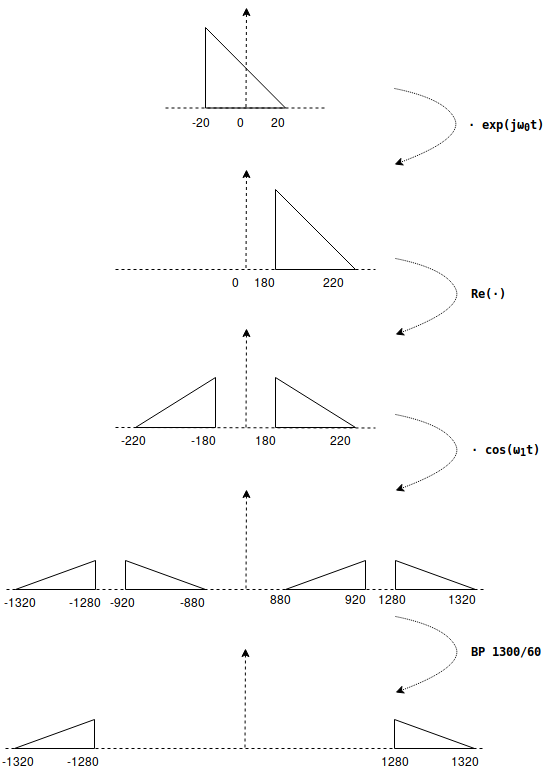
\includegraphics{TPE-ej4.png}
\caption{TPE-ej4.png}
\end{figure}

    \hypertarget{ejercicio-5}{%
\subsection*{Ejercicio 5}\label{ejercicio-5}}

    Realizamos algo similar al ejercicio anterior pero con el proceso de
recepción de los ecos (ignorando el ruido que pueda llegar al sensor): \\

\begin{figure}
\centering
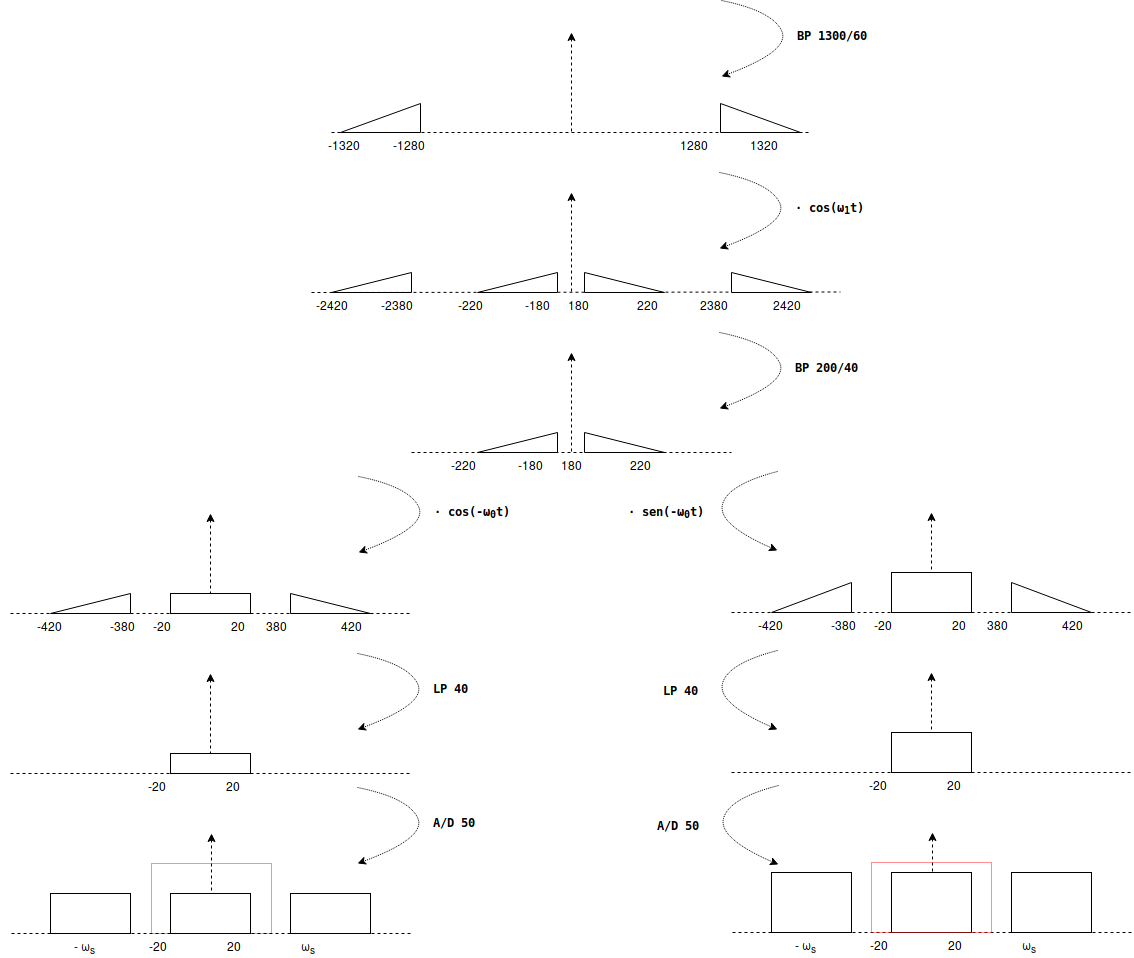
\includegraphics{TPE-ej5.png}
\caption{TPE-ej5.png}
\end{figure}

    \hypertarget{ejercicio-6}{%
\subsection*{Ejercicio 6}\label{ejercicio-6}}

    Para ver la relación, graficamos los espectros de la parte real y de la
parte imaginaria del \emph{chirp}: \\

    \begin{tcolorbox}[breakable, size=fbox, boxrule=1pt, pad at break*=1mm,colback=cellbackground, colframe=cellborder]
\prompt{In}{incolor}{16}{\hspace{4pt}}
\begin{Verbatim}[commandchars=\\\{\}]
\PY{n}{spect\PYZus{}re} \PY{o}{=} \PY{n}{sp\PYZus{}fft}\PY{o}{.}\PY{n}{fft}\PY{p}{(}\PY{n}{np}\PY{o}{.}\PY{n}{real}\PY{p}{(}\PY{n}{chirp}\PY{p}{)}\PY{p}{)}
\PY{n}{spect\PYZus{}im} \PY{o}{=} \PY{n}{sp\PYZus{}fft}\PY{o}{.}\PY{n}{fft}\PY{p}{(}\PY{n}{np}\PY{o}{.}\PY{n}{imag}\PY{p}{(}\PY{n}{chirp}\PY{p}{)}\PY{p}{)}
\PY{n}{freqs\PYZus{}re} \PY{o}{=} \PY{n}{sp\PYZus{}fft}\PY{o}{.}\PY{n}{fftfreq}\PY{p}{(}\PY{n+nb}{len}\PY{p}{(}\PY{n}{spect\PYZus{}re}\PY{p}{)}\PY{p}{,} \PY{l+m+mi}{1} \PY{o}{/} \PY{n}{f\PYZus{}s}\PY{p}{)}
\PY{n}{freqs\PYZus{}im} \PY{o}{=} \PY{n}{sp\PYZus{}fft}\PY{o}{.}\PY{n}{fftfreq}\PY{p}{(}\PY{n+nb}{len}\PY{p}{(}\PY{n}{spect\PYZus{}im}\PY{p}{)}\PY{p}{,} \PY{l+m+mi}{1} \PY{o}{/} \PY{n}{f\PYZus{}s}\PY{p}{)}
\end{Verbatim}
\end{tcolorbox}

    \begin{tcolorbox}[breakable, size=fbox, boxrule=1pt, pad at break*=1mm,colback=cellbackground, colframe=cellborder]
\prompt{In}{incolor}{17}{\hspace{4pt}}
\begin{Verbatim}[commandchars=\\\{\}]
\PY{n}{fig} \PY{o}{=} \PY{n}{plt}\PY{o}{.}\PY{n}{figure}\PY{p}{(}\PY{n}{figsize}\PY{o}{=}\PY{p}{(}\PY{l+m+mi}{12}\PY{p}{,}\PY{l+m+mi}{6}\PY{p}{)}\PY{p}{)}
\PY{n}{fig}\PY{o}{.}\PY{n}{add\PYZus{}subplot}\PY{p}{(}\PY{l+m+mi}{221}\PY{p}{)}
\PY{n}{plt}\PY{o}{.}\PY{n}{plot}\PY{p}{(}\PY{n}{freqs\PYZus{}re}\PY{p}{,} \PY{n}{np}\PY{o}{.}\PY{n}{log10}\PY{p}{(}\PY{n}{np}\PY{o}{.}\PY{n}{abs}\PY{p}{(}\PY{n}{spect\PYZus{}re}\PY{p}{)}\PY{p}{)}\PY{p}{)}
\PY{n}{plt}\PY{o}{.}\PY{n}{xlabel}\PY{p}{(}\PY{l+s+s1}{\PYZsq{}}\PY{l+s+s1}{\PYZdl{}f\PYZdl{} [MHz]}\PY{l+s+s1}{\PYZsq{}}\PY{p}{)}
\PY{n}{plt}\PY{o}{.}\PY{n}{title}\PY{p}{(}\PY{l+s+s2}{\PYZdq{}}\PY{l+s+s2}{Espectro del \PYZdl{}chirp\PYZdl{} (parte real)}\PY{l+s+s2}{\PYZdq{}}\PY{p}{)}\PY{p}{;}
\PY{n}{fig}\PY{o}{.}\PY{n}{add\PYZus{}subplot}\PY{p}{(}\PY{l+m+mi}{222}\PY{p}{)}
\PY{n}{plt}\PY{o}{.}\PY{n}{plot}\PY{p}{(}\PY{n}{freqs\PYZus{}im}\PY{p}{,} \PY{n}{np}\PY{o}{.}\PY{n}{log10}\PY{p}{(}\PY{n}{np}\PY{o}{.}\PY{n}{abs}\PY{p}{(}\PY{n}{spect\PYZus{}im}\PY{p}{)}\PY{p}{)}\PY{p}{)}
\PY{n}{plt}\PY{o}{.}\PY{n}{xlabel}\PY{p}{(}\PY{l+s+s1}{\PYZsq{}}\PY{l+s+s1}{\PYZdl{}f\PYZdl{} [MHz]}\PY{l+s+s1}{\PYZsq{}}\PY{p}{)}
\PY{n}{plt}\PY{o}{.}\PY{n}{title}\PY{p}{(}\PY{l+s+s2}{\PYZdq{}}\PY{l+s+s2}{Espectro del \PYZdl{}chirp\PYZdl{} (parte imaginaria)}\PY{l+s+s2}{\PYZdq{}}\PY{p}{)}\PY{p}{;}
\end{Verbatim}
\end{tcolorbox}

    \begin{center}
    \adjustimage{max size={0.9\linewidth}{0.9\paperheight}}{output_38_0.png}
    \end{center}
    { \hspace*{\fill} \\}
    
    Descontando las oscilaciones y picos muy rápidos que se generan por el
fenómeno de Gibbs, se puede reconocer \(I(n)\) y \(Q(n)\) (del ejercicio
anterior) en las figuras. \\

    \hypertarget{ejercicio-7}{%
\subsection*{Ejercicio 7}\label{ejercicio-7}}

    La operación de correlación se ve muy similar a la de convolución.
Desarrollando la expresión dada:
\[ C_{xy}(n) = x(n) \star y(n) = \sum_{k} x^*(k) y(k+n) = [x^*(n)] \ast [y(-n)] \neq C_{yx}(n) \]
Con esto vemos que la operación no es conmutativa. Esto último también
nos permite expresar la correlación en términos de transformadas de
Fourier:
\[ C_{xy} = \mathcal{F}^{-1}[\mathcal{F}^*[x] \mathcal{F}[y]] \]

    \hypertarget{ejercicio-8}{%
\subsection*{Ejercicio 8}\label{ejercicio-8}}

    Calculamos la autocorrelación del \emph{chirp} usando la expresión del
ejercicio anterior y graficamos: \\

    \begin{tcolorbox}[breakable, size=fbox, boxrule=1pt, pad at break*=1mm,colback=cellbackground, colframe=cellborder]
\prompt{In}{incolor}{18}{\hspace{4pt}}
\begin{Verbatim}[commandchars=\\\{\}]
\PY{n}{chirp\PYZus{}autocorr} \PY{o}{=} \PY{n}{np}\PY{o}{.}\PY{n}{convolve}\PY{p}{(}\PY{n}{np}\PY{o}{.}\PY{n}{conj}\PY{p}{(}\PY{n}{chirp}\PY{p}{)}\PY{p}{,} \PY{n}{chirp}\PY{p}{[}\PY{p}{:}\PY{p}{:}\PY{o}{\PYZhy{}}\PY{l+m+mi}{1}\PY{p}{]}\PY{p}{)}
\end{Verbatim}
\end{tcolorbox}

    \begin{tcolorbox}[breakable, size=fbox, boxrule=1pt, pad at break*=1mm,colback=cellbackground, colframe=cellborder]
\prompt{In}{incolor}{19}{\hspace{4pt}}
\begin{Verbatim}[commandchars=\\\{\}]
\PY{n}{plt}\PY{o}{.}\PY{n}{figure}\PY{p}{(}\PY{n}{figsize}\PY{o}{=}\PY{p}{(}\PY{l+m+mi}{8}\PY{p}{,}\PY{l+m+mi}{4}\PY{p}{)}\PY{p}{)}
\PY{n}{plt}\PY{o}{.}\PY{n}{plot}\PY{p}{(}\PY{n}{np}\PY{o}{.}\PY{n}{linspace}\PY{p}{(}\PY{l+m+mi}{-T_{rg}/2}\PY{p}{,} \PY{n}{T_{rg}/2}\PY{p}{,} \PY{n}{chirp\PYZus{}autocorr}\PY{o}{.}\PY{n}{size}\PY{p}{)}\PY{p}{,} \PY{n}{np}\PY{o}{.}\PY{n}{abs}\PY{p}{(}\PY{n}{chirp\PYZus{}autocorr}\PY{p}{)}\PY{p}{)}
\PY{n}{plt}\PY{o}{.}\PY{n}{title}\PY{p}{(}\PY{l+s+s2}{\PYZdq{}}\PY{l+s+s2}{Autocorrelación del \PYZdl{}chirp\PYZdl{}}\PY{l+s+s2}{\PYZdq{}}\PY{p}{)}
\PY{n}{plt}\PY{o}{.}\PY{n}{xlabel}\PY{p}{(}\PY{l+s+s1}{\PYZsq{}}\PY{l+s+s1}{\PYZdl{}t\PYZdl{} [\PYZdl{}}\PY{l+s+s1}{\PYZbs{}}\PY{l+s+s1}{mu\PYZdl{}s]}\PY{l+s+s1}{\PYZsq{}}\PY{p}{)}\PY{p}{;}
\end{Verbatim}
\end{tcolorbox}

    \begin{center}
    \adjustimage{max size={0.9\linewidth}{0.9\paperheight}}{output_45_0.png}
    \end{center}
    { \hspace*{\fill} \\}
    
    El factor de compresión es aproximadamente de $T \cdot BW = 380$. \\

    \hypertarget{ejercicio-9}{%
\subsection*{Ejercicio 9}\label{ejercicio-9}}

    Repetimos la autocorrelación pero mediante DFT. Antes de realizar la
cuenta nos aseguramos de que el resultado salga como queremos agregando
\emph{padding} de cada lado en las copias del \emph{chirp}. \\

    \begin{tcolorbox}[breakable, size=fbox, boxrule=1pt, pad at break*=1mm,colback=cellbackground, colframe=cellborder]
\prompt{In}{incolor}{20}{\hspace{4pt}}
\begin{Verbatim}[commandchars=\\\{\}]
\PY{n}{chirp\PYZus{}a} \PY{o}{=} \PY{n}{np}\PY{o}{.}\PY{n}{pad}\PY{p}{(}\PY{n}{chirp}\PY{p}{,} \PY{p}{(}\PY{l+m+mi}{0}\PY{p}{,} \PY{n+nb}{len}\PY{p}{(}\PY{n}{chirp}\PY{p}{)} \PY{o}{\PYZhy{}} \PY{l+m+mi}{1}\PY{p}{)}\PY{p}{,} \PY{n}{mode}\PY{o}{=}\PY{l+s+s1}{\PYZsq{}}\PY{l+s+s1}{constant}\PY{l+s+s1}{\PYZsq{}}\PY{p}{)}
\PY{n}{chirp\PYZus{}b} \PY{o}{=} \PY{n}{np}\PY{o}{.}\PY{n}{pad}\PY{p}{(}\PY{n}{chirp}\PY{p}{,} \PY{p}{(}\PY{n+nb}{len}\PY{p}{(}\PY{n}{chirp}\PY{p}{)} \PY{o}{\PYZhy{}} \PY{l+m+mi}{1}\PY{p}{,} \PY{l+m+mi}{0}\PY{p}{)}\PY{p}{,} \PY{n}{mode}\PY{o}{=}\PY{l+s+s1}{\PYZsq{}}\PY{l+s+s1}{constant}\PY{l+s+s1}{\PYZsq{}}\PY{p}{)}
\PY{c+c1}{\PYZsh{} Ver ecuación en el Ejercicio 7}
\PY{n}{chirp\PYZus{}autocorr\PYZus{}2} \PY{o}{=} \PY{n}{sp\PYZus{}fft}\PY{o}{.}\PY{n}{ifft}\PY{p}{(}\PY{n}{np}\PY{o}{.}\PY{n}{conj}\PY{p}{(}\PY{n}{sp\PYZus{}fft}\PY{o}{.}\PY{n}{fft}\PY{p}{(}\PY{n}{chirp\PYZus{}a}\PY{p}{)}\PY{p}{)} \PY{o}{*} \PY{n}{sp\PYZus{}fft}\PY{o}{.}\PY{n}{fft}\PY{p}{(}\PY{n}{chirp\PYZus{}b}\PY{p}{)}\PY{p}{)}
\end{Verbatim}
\end{tcolorbox}

    \begin{tcolorbox}[breakable, size=fbox, boxrule=1pt, pad at break*=1mm,colback=cellbackground, colframe=cellborder]
\prompt{In}{incolor}{21}{\hspace{4pt}}
\begin{Verbatim}[commandchars=\\\{\}]
\PY{n}{plt}\PY{o}{.}\PY{n}{figure}\PY{p}{(}\PY{n}{figsize}\PY{o}{=}\PY{p}{(}\PY{l+m+mi}{8}\PY{p}{,}\PY{l+m+mi}{4}\PY{p}{)}\PY{p}{)}
\PY{n}{plt}\PY{o}{.}\PY{n}{plot}\PY{p}{(}\PY{n}{np}\PY{o}{.}\PY{n}{linspace}\PY{p}{(}\PY{l+m+mi}{-T_{rg}/2}\PY{p}{,} \PY{n}{T_{rg}/2}\PY{p}{,} \PY{n}{chirp\PYZus{}autocorr\PYZus{}2}\PY{o}{.}\PY{n}{size}\PY{p}{)}\PY{p}{,} \PY{n}{np}\PY{o}{.}\PY{n}{abs}\PY{p}{(}\PY{n}{chirp\PYZus{}autocorr\PYZus{}2}\PY{p}{)}\PY{p}{)}
\PY{c+c1}{\PYZsh{} plt.plot(np.abs(chirp\PYZus{}autocorr\PYZus{}2))}
\PY{n}{plt}\PY{o}{.}\PY{n}{title}\PY{p}{(}\PY{l+s+s2}{\PYZdq{}}\PY{l+s+s2}{Autocorrelación del \PYZdl{}chirp\PYZdl{} (mediante T de F)}\PY{l+s+s2}{\PYZdq{}}\PY{p}{)}
\PY{n}{plt}\PY{o}{.}\PY{n}{xlabel}\PY{p}{(}\PY{l+s+s1}{\PYZsq{}}\PY{l+s+s1}{\PYZdl{}t\PYZdl{} [\PYZdl{}}\PY{l+s+s1}{\PYZbs{}}\PY{l+s+s1}{mu\PYZdl{}s]}\PY{l+s+s1}{\PYZsq{}}\PY{p}{)}\PY{p}{;}
\end{Verbatim}
\end{tcolorbox}

    \begin{center}
    \adjustimage{max size={0.9\linewidth}{0.9\paperheight}}{output_50_0.png}
    \end{center}
    { \hspace*{\fill} \\}
    
    \hypertarget{ejercicio-10}{%
\subsection*{Ejercicio 10}\label{ejercicio-10}}

    Cargamos la matriz de la imagen sintética desde el archivo provisto: \\

    \begin{tcolorbox}[breakable, size=fbox, boxrule=1pt, pad at break*=1mm,colback=cellbackground, colframe=cellborder]
\prompt{In}{incolor}{22}{\hspace{4pt}}
\begin{Verbatim}[commandchars=\\\{\}]
\PY{n}{sint\PYZus{}mat} \PY{o}{=} \PY{n}{sp\PYZus{}io}\PY{o}{.}\PY{n}{loadmat}\PY{p}{(}\PY{l+s+s1}{\PYZsq{}}\PY{l+s+s1}{SAR\PYZus{}data\PYZus{}sint.mat}\PY{l+s+s1}{\PYZsq{}}\PY{p}{)}\PY{p}{[}\PY{l+s+s1}{\PYZsq{}}\PY{l+s+s1}{data\PYZus{}sint}\PY{l+s+s1}{\PYZsq{}}\PY{p}{]}
\end{Verbatim}
\end{tcolorbox}

    \begin{tcolorbox}[breakable, size=fbox, boxrule=1pt, pad at break*=1mm,colback=cellbackground, colframe=cellborder]
\prompt{In}{incolor}{23}{\hspace{4pt}}
\begin{Verbatim}[commandchars=\\\{\}]
\PY{n}{plt}\PY{o}{.}\PY{n}{rcParams}\PY{p}{[}\PY{l+s+s2}{\PYZdq{}}\PY{l+s+s2}{figure.figsize}\PY{l+s+s2}{\PYZdq{}}\PY{p}{]}\PY{p}{[}\PY{l+m+mi}{1}\PY{p}{]} \PY{o}{=} \PY{l+m+mi}{6}
\PY{n}{plt}\PY{o}{.}\PY{n}{figure}\PY{p}{(}\PY{p}{)}\PY{o}{.}\PY{n}{add\PYZus{}subplot}\PY{p}{(}\PY{l+m+mi}{111}\PY{p}{)}\PY{o}{.}\PY{n}{set\PYZus{}aspect}\PY{p}{(}\PY{l+s+s1}{\PYZsq{}}\PY{l+s+s1}{equal}\PY{l+s+s1}{\PYZsq{}}\PY{p}{,} \PY{l+s+s1}{\PYZsq{}}\PY{l+s+s1}{box}\PY{l+s+s1}{\PYZsq{}}\PY{p}{)}
\PY{n}{plt}\PY{o}{.}\PY{n}{pcolormesh}\PY{p}{(}\PY{n+nb}{abs}\PY{p}{(}\PY{n}{sint\PYZus{}mat}\PY{p}{)}\PY{p}{,} \PY{n}{cmap}\PY{o}{=}\PY{n}{cm}\PY{o}{.}\PY{n}{gray}\PY{p}{)}
\PY{n}{plt}\PY{o}{.}\PY{n}{title}\PY{p}{(}\PY{l+s+s2}{\PYZdq{}}\PY{l+s+s2}{Imagen sintética en matriz}\PY{l+s+s2}{\PYZdq{}}\PY{p}{)}\PY{p}{;}
\end{Verbatim}
\end{tcolorbox}

    \begin{center}
    \adjustimage{max size={0.9\linewidth}{0.9\paperheight}}{output_54_0.png}
    \end{center}
    { \hspace*{\fill} \\}
    
    Ahora aplicamos el enfocado en rango, realizando la correlación de cada
fila de la matriz con el \emph{chirp} emitido: \\

    \begin{tcolorbox}[breakable, size=fbox, boxrule=1pt, pad at break*=1mm,colback=cellbackground, colframe=cellborder]
\prompt{In}{incolor}{24}{\hspace{4pt}}
\begin{Verbatim}[commandchars=\\\{\}]
\PY{k}{def} \PY{n+nf}{correlation}\PY{p}{(}\PY{n}{x}\PY{p}{,} \PY{n}{y}\PY{p}{)}\PY{p}{:}
    \PY{n}{x} \PY{o}{=} \PY{n}{np}\PY{o}{.}\PY{n}{pad}\PY{p}{(}\PY{n}{x}\PY{p}{,} \PY{p}{(}\PY{l+m+mi}{0}\PY{p}{,} \PY{n+nb}{len}\PY{p}{(}\PY{n}{y}\PY{p}{)} \PY{o}{\PYZhy{}} \PY{n+nb}{len}\PY{p}{(}\PY{n}{x}\PY{p}{)}\PY{p}{)}\PY{p}{,} \PY{n}{mode}\PY{o}{=}\PY{l+s+s1}{\PYZsq{}}\PY{l+s+s1}{constant}\PY{l+s+s1}{\PYZsq{}}\PY{p}{)}
    \PY{k}{return} \PY{n}{sp\PYZus{}fft}\PY{o}{.}\PY{n}{ifft}\PY{p}{(}\PY{n}{np}\PY{o}{.}\PY{n}{conj}\PY{p}{(}\PY{n}{sp\PYZus{}fft}\PY{o}{.}\PY{n}{fft}\PY{p}{(}\PY{n}{x}\PY{p}{)}\PY{p}{)} \PY{o}{*} \PY{n}{sp\PYZus{}fft}\PY{o}{.}\PY{n}{fft}\PY{p}{(}\PY{n}{y}\PY{p}{)}\PY{p}{)}

\PY{k}{def} \PY{n+nf}{range\PYZus{}compression}\PY{p}{(}\PY{n}{mat}\PY{p}{,} \PY{n}{chirp\PYZus{}signal}\PY{p}{)}\PY{p}{:}
    \PY{k}{return} \PY{n}{np}\PY{o}{.}\PY{n}{array}\PY{p}{(}\PY{p}{[}\PY{n}{correlation}\PY{p}{(}\PY{n}{chirp\PYZus{}signal}\PY{p}{,} \PY{n}{row}\PY{p}{)} \PY{k}{for} \PY{n}{row} \PY{o+ow}{in} \PY{n}{mat}\PY{p}{]}\PY{p}{)}
\end{Verbatim}
\end{tcolorbox}

    \begin{tcolorbox}[breakable, size=fbox, boxrule=1pt, pad at break*=1mm,colback=cellbackground, colframe=cellborder]
\prompt{In}{incolor}{25}{\hspace{4pt}}
\begin{Verbatim}[commandchars=\\\{\}]
\PY{n}{sint\PYZus{}range\PYZus{}compressed} \PY{o}{=} \PY{n}{range\PYZus{}compression}\PY{p}{(}\PY{n}{sint\PYZus{}mat}\PY{p}{,} \PY{n}{chirp}\PY{p}{)}
\end{Verbatim}
\end{tcolorbox}

    \begin{tcolorbox}[breakable, size=fbox, boxrule=1pt, pad at break*=1mm,colback=cellbackground, colframe=cellborder]
\prompt{In}{incolor}{26}{\hspace{4pt}}
\begin{Verbatim}[commandchars=\\\{\}]
\PY{n}{fig} \PY{o}{=} \PY{n}{plt}\PY{o}{.}\PY{n}{figure}\PY{p}{(}\PY{n}{figsize}\PY{o}{=}\PY{p}{(}\PY{l+m+mi}{13}\PY{p}{,}\PY{l+m+mi}{13}\PY{p}{)}\PY{p}{)}
\PY{n}{fig}\PY{o}{.}\PY{n}{add\PYZus{}subplot}\PY{p}{(}\PY{l+m+mi}{221}\PY{p}{)}\PY{o}{.}\PY{n}{set\PYZus{}aspect}\PY{p}{(}\PY{l+s+s1}{\PYZsq{}}\PY{l+s+s1}{equal}\PY{l+s+s1}{\PYZsq{}}\PY{p}{,} \PY{l+s+s1}{\PYZsq{}}\PY{l+s+s1}{box}\PY{l+s+s1}{\PYZsq{}}\PY{p}{)}
\PY{n}{plt}\PY{o}{.}\PY{n}{pcolormesh}\PY{p}{(}\PY{n+nb}{abs}\PY{p}{(}\PY{n}{sint\PYZus{}range\PYZus{}compressed}\PY{p}{)}\PY{p}{,} \PY{n}{cmap}\PY{o}{=}\PY{n}{cm}\PY{o}{.}\PY{n}{gray}\PY{p}{)}
\PY{n}{plt}\PY{o}{.}\PY{n}{title}\PY{p}{(}\PY{l+s+s2}{\PYZdq{}}\PY{l+s+s2}{Imagen sintética enfocada en rango}\PY{l+s+s2}{\PYZdq{}}\PY{p}{)}\PY{p}{;}
\PY{n}{ax} \PY{o}{=} \PY{n}{fig}\PY{o}{.}\PY{n}{add\PYZus{}subplot}\PY{p}{(}\PY{l+m+mi}{222}\PY{p}{)}
\PY{n}{plt}\PY{o}{.}\PY{n}{axis}\PY{p}{(}\PY{p}{[}\PY{l+m+mi}{600}\PY{p}{,} \PY{l+m+mi}{700}\PY{p}{,} \PY{l+m+mi}{1500}\PY{p}{,} \PY{l+m+mi}{2700}\PY{p}{]}\PY{p}{)}
\PY{n}{plt}\PY{o}{.}\PY{n}{pcolormesh}\PY{p}{(}\PY{n+nb}{abs}\PY{p}{(}\PY{n}{sint\PYZus{}range\PYZus{}compressed}\PY{p}{)}\PY{p}{,} \PY{n}{cmap}\PY{o}{=}\PY{n}{cm}\PY{o}{.}\PY{n}{gray}\PY{p}{)}
\PY{n}{plt}\PY{o}{.}\PY{n}{title}\PY{p}{(}\PY{l+s+s2}{\PYZdq{}}\PY{l+s+s2}{Imagen sintética enfocada en rango (detalle)}\PY{l+s+s2}{\PYZdq{}}\PY{p}{)}\PY{p}{;}
\end{Verbatim}
\end{tcolorbox}

    \begin{center}
    \adjustimage{max size={0.9\linewidth}{0.9\paperheight}}{output_58_0.png}
    \end{center}
    { \hspace*{\fill} \\}
    
    Es bastante tenue pero se puede apreciar una línea borroneada por la
columna 650. Ahora hacemos un proceso similar para la imagen captada por
SARAT. Para graficar usamos el logaritmo y transponemos por comodidad. \\

    \begin{tcolorbox}[breakable, size=fbox, boxrule=1pt, pad at break*=1mm,colback=cellbackground, colframe=cellborder]
\prompt{In}{incolor}{27}{\hspace{4pt}}
\begin{Verbatim}[commandchars=\\\{\}]
\PY{n}{sarat\PYZus{}mat} \PY{o}{=} \PY{n}{sp\PYZus{}io}\PY{o}{.}\PY{n}{loadmat}\PY{p}{(}\PY{l+s+s1}{\PYZsq{}}\PY{l+s+s1}{SAR\PYZus{}data\PYZus{}sarat.mat}\PY{l+s+s1}{\PYZsq{}}\PY{p}{)}\PY{p}{[}\PY{l+s+s1}{\PYZsq{}}\PY{l+s+s1}{data}\PY{l+s+s1}{\PYZsq{}}\PY{p}{]}
\end{Verbatim}
\end{tcolorbox}

    \begin{tcolorbox}[breakable, size=fbox, boxrule=1pt, pad at break*=1mm,colback=cellbackground, colframe=cellborder]
\prompt{In}{incolor}{28}{\hspace{4pt}}
\begin{Verbatim}[commandchars=\\\{\}]
\PY{n}{plt}\PY{o}{.}\PY{n}{figure}\PY{p}{(}\PY{n}{figsize}\PY{o}{=}\PY{p}{(}\PY{l+m+mi}{12}\PY{p}{,} \PY{l+m+mi}{6}\PY{p}{)}\PY{p}{)}\PY{o}{.}\PY{n}{add\PYZus{}subplot}\PY{p}{(}\PY{l+m+mi}{111}\PY{p}{)}
\PY{n}{plt}\PY{o}{.}\PY{n}{pcolormesh}\PY{p}{(}\PY{n}{np}\PY{o}{.}\PY{n}{log10}\PY{p}{(}\PY{n}{np}\PY{o}{.}\PY{n}{abs}\PY{p}{(}\PY{n}{np}\PY{o}{.}\PY{n}{transpose}\PY{p}{(}\PY{n}{sarat\PYZus{}mat}\PY{p}{)}\PY{p}{)}\PY{p}{)}\PY{p}{,} \PY{n}{cmap}\PY{o}{=}\PY{n}{cm}\PY{o}{.}\PY{n}{gray}\PY{p}{)}
\PY{n}{plt}\PY{o}{.}\PY{n}{title}\PY{p}{(}\PY{l+s+s2}{\PYZdq{}}\PY{l+s+s2}{Imagen SARAT en archivo}\PY{l+s+s2}{\PYZdq{}}\PY{p}{)}\PY{p}{;}
\end{Verbatim}
\end{tcolorbox}

    \begin{center}
    \adjustimage{max size={0.9\linewidth}{0.9\paperheight}}{output_61_0.png}
    \end{center}
    { \hspace*{\fill} \\}
    
    \begin{tcolorbox}[breakable, size=fbox, boxrule=1pt, pad at break*=1mm,colback=cellbackground, colframe=cellborder]
\prompt{In}{incolor}{29}{\hspace{4pt}}
\begin{Verbatim}[commandchars=\\\{\}]
\PY{n}{sarat\PYZus{}range\PYZus{}compressed} \PY{o}{=} \PY{n}{range\PYZus{}compression}\PY{p}{(}\PY{n}{sarat\PYZus{}mat}\PY{p}{,} \PY{n}{chirp}\PY{p}{)}
\end{Verbatim}
\end{tcolorbox}

    \begin{tcolorbox}[breakable, size=fbox, boxrule=1pt, pad at break*=1mm,colback=cellbackground, colframe=cellborder]
\prompt{In}{incolor}{30}{\hspace{4pt}}
\begin{Verbatim}[commandchars=\\\{\}]
\PY{n}{plt}\PY{o}{.}\PY{n}{figure}\PY{p}{(}\PY{n}{figsize}\PY{o}{=}\PY{p}{(}\PY{l+m+mi}{12}\PY{p}{,} \PY{l+m+mi}{6}\PY{p}{)}\PY{p}{)}\PY{o}{.}\PY{n}{add\PYZus{}subplot}\PY{p}{(}\PY{l+m+mi}{111}\PY{p}{)}
\PY{n}{plt}\PY{o}{.}\PY{n}{pcolormesh}\PY{p}{(}\PY{n}{np}\PY{o}{.}\PY{n}{log10}\PY{p}{(}\PY{n}{np}\PY{o}{.}\PY{n}{abs}\PY{p}{(}\PY{n}{np}\PY{o}{.}\PY{n}{transpose}\PY{p}{(}\PY{n}{sarat\PYZus{}range\PYZus{}compressed}\PY{p}{)}\PY{p}{)}\PY{p}{)}\PY{p}{,} \PY{n}{cmap}\PY{o}{=}\PY{n}{cm}\PY{o}{.}\PY{n}{gray}\PY{p}{)}
\PY{n}{plt}\PY{o}{.}\PY{n}{title}\PY{p}{(}\PY{l+s+s2}{\PYZdq{}}\PY{l+s+s2}{Imagen SARAT enfocada en rango}\PY{l+s+s2}{\PYZdq{}}\PY{p}{)}\PY{p}{;}
\end{Verbatim}
\end{tcolorbox}

    \begin{center}
    \adjustimage{max size={0.9\linewidth}{0.9\paperheight}}{output_63_0.png}
    \end{center}
    { \hspace*{\fill} \\}
    
    Se empieza a apreciar formas en la imagen, pero todavía quedará enfocar
en el eje de acimut.

    \hypertarget{ejercicio-11}{%
\subsection*{Ejercicio 11}\label{ejercicio-11}}

    Usamos las ecuaciones y constantes dadas para calcular la duración
temporal del nuevo \emph{chirp}: \\

    \begin{tcolorbox}[breakable, size=fbox, boxrule=1pt, pad at break*=1mm,colback=cellbackground, colframe=cellborder]
\prompt{In}{incolor}{ }{\hspace{4pt}}
\begin{Verbatim}[commandchars=\\\{\}]
\PY{n}{T\PYZus{}az} \PY{o}{=} \PY{n}{eta\PYZus{}az} \PY{o}{*} \PY{n}{r\PYZus{}0} \PY{o}{/} \PY{n}{nu}
\end{Verbatim}
\end{tcolorbox}

    Con lo que tenemos $T_{az} = 7.4751 \mu$s.

Para el ancho de banda, tal como hicimos al principio del trabajo,
derivamos la fase y aplicamos entre \(-T_{az}/2\) y \(T_{az}/2\):
\[ f_{az}(t) = -2 \frac{\nu^2}{\lambda r_0} t \] \\

    \begin{tcolorbox}[breakable, size=fbox, boxrule=1pt, pad at break*=1mm,colback=cellbackground, colframe=cellborder]
\prompt{In}{incolor}{ }{\hspace{4pt}}
\begin{Verbatim}[commandchars=\\\{\}]
\PY{n}{frec\PYZus{}az} \PY{o}{=} \PY{k}{lambda} \PY{n}{x}\PY{p}{:} \PY{o}{\PYZhy{}}\PY{l+m+mi}{2} \PY{o}{*} \PY{n}{nu}\PY{o}{*}\PY{o}{*}\PY{l+m+mi}{2} \PY{o}{*} \PY{n}{x} \PY{o}{/} \PY{p}{(}\PY{n}{lamb} \PY{o}{*} \PY{n}{r\PYZus{}0}\PY{p}{)}
\PY{n}{bw\PYZus{}az} \PY{o}{=} \PY{n+nb}{abs}\PY{p}{(}\PY{n}{frec\PYZus{}az}\PY{p}{(}\PY{o}{\PYZhy{}}\PY{n}{T\PYZus{}az}\PY{o}{/}\PY{l+m+mi}{2}\PY{p}{)} \PY{o}{\PYZhy{}} \PY{n}{frec\PYZus{}az}\PY{p}{(}\PY{n}{T\PYZus{}az}\PY{o}{/}\PY{l+m+mi}{2}\PY{p}{)}\PY{p}{)}
\end{Verbatim}
\end{tcolorbox}

    Con lo que tenemos $BW_{az} = 100.487$ Hz. \\

    \hypertarget{ejercicio-12}{%
\subsection*{Ejercicio 12}\label{ejercicio-12}}

    \begin{tcolorbox}[breakable, size=fbox, boxrule=1pt, pad at break*=1mm,colback=cellbackground, colframe=cellborder]
\prompt{In}{incolor}{33}{\hspace{4pt}}
\begin{Verbatim}[commandchars=\\\{\}]
\PY{n}{t\PYZus{}az} \PY{o}{=} \PY{n}{np}\PY{o}{.}\PY{n}{linspace}\PY{p}{(}\PY{o}{\PYZhy{}}\PY{n}{T\PYZus{}az}\PY{o}{/}\PY{l+m+mi}{2}\PY{p}{,} \PY{n}{T\PYZus{}az}\PY{o}{/}\PY{l+m+mi}{2}\PY{p}{,} \PY{n+nb}{int}\PY{p}{(}\PY{n}{prf} \PY{o}{*} \PY{n}{T\PYZus{}az}\PY{p}{)}\PY{p}{,} \PY{n}{endpoint}\PY{o}{=}\PY{k+kc}{False}\PY{p}{)}

\PY{n}{k\PYZus{}1} \PY{o}{=} \PY{o}{\PYZhy{}}\PY{n}{nu}\PY{o}{*}\PY{o}{*}\PY{l+m+mi}{2} \PY{o}{/} \PY{p}{(}\PY{n}{lamb} \PY{o}{*} \PY{n}{r\PYZus{}0}\PY{p}{)}
\PY{n}{k\PYZus{}2} \PY{o}{=} \PY{l+m+mi}{0}
\PY{n}{chirp\PYZus{}az\PYZus{}ph} \PY{o}{=} \PY{k}{lambda} \PY{n}{x}\PY{p}{:} \PY{n}{k\PYZus{}1} \PY{o}{*} \PY{n}{x}\PY{o}{*}\PY{o}{*}\PY{l+m+mi}{2} \PY{o}{+} \PY{n}{k\PYZus{}2} \PY{o}{*} \PY{n}{x} \PY{o}{+} \PY{n}{phi\PYZus{}0}

\PY{n}{chirp\PYZus{}az} \PY{o}{=} \PY{n}{np}\PY{o}{.}\PY{n}{array}\PY{p}{(}\PY{p}{[}\PY{n}{np}\PY{o}{.}\PY{n}{exp}\PY{p}{(}\PY{l+m+mi}{2}\PY{n}{j} \PY{o}{*} \PY{n}{np}\PY{o}{.}\PY{n}{pi} \PY{o}{*} \PY{n}{chirp\PYZus{}az\PYZus{}ph}\PY{p}{(}\PY{n}{x}\PY{p}{)}\PY{p}{)} \PY{k}{for} \PY{n}{x} \PY{o+ow}{in} \PY{n}{t\PYZus{}az}\PY{p}{]}\PY{p}{)}
\PY{c+c1}{\PYZsh{}\PYZsh{} Forma alternativa:}
\PY{c+c1}{\PYZsh{} f0\PYZus{}az = frec\PYZus{}az(\PYZhy{}T\PYZus{}az/2)}
\PY{c+c1}{\PYZsh{} f1\PYZus{}az = frec\PYZus{}az( T\PYZus{}az/2)}
\PY{c+c1}{\PYZsh{} chirp\PYZus{}az\PYZus{}re =      sp\PYZus{}signal.chirp(t\PYZus{}az, f0=f0\PYZus{}az, f1=f1\PYZus{}az, t1=T\PYZus{}az)}
\PY{c+c1}{\PYZsh{} chirp\PYZus{}az\PYZus{}im = 1j * sp\PYZus{}signal.chirp(t\PYZus{}az, f0=f0\PYZus{}az, f1=f1\PYZus{}az, t1=T\PYZus{}az, phi=\PYZhy{}90)}
\PY{c+c1}{\PYZsh{} chirp\PYZus{}az = chirp\PYZus{}az\PYZus{}re + chirp\PYZus{}az\PYZus{}im}
\end{Verbatim}
\end{tcolorbox}

    Nuevamente podemos graficar la función de fase y verificamos que ahora
varía en forma descendente: \\

    \begin{tcolorbox}[breakable, size=fbox, boxrule=1pt, pad at break*=1mm,colback=cellbackground, colframe=cellborder]
\prompt{In}{incolor}{34}{\hspace{4pt}}
\begin{Verbatim}[commandchars=\\\{\}]
\PY{n}{plt}\PY{o}{.}\PY{n}{figure}\PY{p}{(}\PY{n}{figsize}\PY{o}{=}\PY{p}{(}\PY{l+m+mi}{8}\PY{p}{,}\PY{l+m+mi}{4}\PY{p}{)}\PY{p}{)}
\PY{n}{plt}\PY{o}{.}\PY{n}{plot}\PY{p}{(}\PY{n}{t\PYZus{}az}\PY{p}{,} \PY{p}{[}\PY{n}{chirp\PYZus{}az\PYZus{}ph}\PY{p}{(}\PY{n}{x}\PY{p}{)} \PY{k}{for} \PY{n}{x} \PY{o+ow}{in} \PY{n}{t\PYZus{}az}\PY{p}{]}\PY{p}{)}
\PY{n}{plt}\PY{o}{.}\PY{n}{title}\PY{p}{(}\PY{l+s+s2}{\PYZdq{}}\PY{l+s+s2}{\PYZdl{}Chirp\PYZdl{} acimut, fase}\PY{l+s+s2}{\PYZdq{}}\PY{p}{)}
\PY{n}{plt}\PY{o}{.}\PY{n}{xlabel}\PY{p}{(}\PY{l+s+s1}{\PYZsq{}}\PY{l+s+s1}{\PYZdl{}t\PYZdl{} [\PYZdl{}}\PY{l+s+s1}{\PYZbs{}}\PY{l+s+s1}{mu\PYZdl{}s]}\PY{l+s+s1}{\PYZsq{}}\PY{p}{)}\PY{p}{;}
\end{Verbatim}
\end{tcolorbox}

    \begin{center}
    \adjustimage{max size={0.9\linewidth}{0.9\paperheight}}{output_74_0.png}
    \end{center}
    { \hspace*{\fill} \\}
    
    Veremos el mismo cambio de sentido al graficar el espectograma para este
nuevo \emph{chirp} que usaremos en la línea del acimut: \\

    \begin{tcolorbox}[breakable, size=fbox, boxrule=1pt, pad at break*=1mm,colback=cellbackground, colframe=cellborder]
\prompt{In}{incolor}{35}{\hspace{4pt}}
\begin{Verbatim}[commandchars=\\\{\}]
\PY{n}{freqs\PYZus{}az}\PY{p}{,} \PY{n}{times\PYZus{}az}\PY{p}{,} \PY{n}{spect\PYZus{}az} \PY{o}{=} \PY{n}{sp\PYZus{}signal}\PY{o}{.}\PY{n}{spectrogram}\PY{p}{(}\PY{n}{chirp\PYZus{}az}\PY{p}{,} \PY{n}{fs}\PY{o}{=}\PY{n}{prf}\PY{p}{,} \PY{n}{nperseg}\PY{o}{=}\PY{l+m+mi}{50}\PY{p}{,} \PY{n}{noverlap}\PY{o}{=}\PY{l+m+mi}{20}\PY{p}{,} \PY{n}{window}\PY{o}{=}\PY{l+s+s1}{\PYZsq{}}\PY{l+s+s1}{boxcar}\PY{l+s+s1}{\PYZsq{}}\PY{p}{,} \PY{n}{return\PYZus{}onesided}\PY{o}{=}\PY{k+kc}{False}\PY{p}{)}
\PY{n}{freqs\PYZus{}az} \PY{o}{=} \PY{n}{sp\PYZus{}fft}\PY{o}{.}\PY{n}{fftshift}\PY{p}{(}\PY{n}{freqs\PYZus{}az}\PY{p}{)}
\PY{n}{spect\PYZus{}az} \PY{o}{=} \PY{n}{sp\PYZus{}fft}\PY{o}{.}\PY{n}{fftshift}\PY{p}{(}\PY{n}{spect\PYZus{}az}\PY{p}{,} \PY{n}{axes}\PY{o}{=}\PY{l+m+mi}{0}\PY{p}{)}
\end{Verbatim}
\end{tcolorbox}

    \begin{tcolorbox}[breakable, size=fbox, boxrule=1pt, pad at break*=1mm,colback=cellbackground, colframe=cellborder]
\prompt{In}{incolor}{36}{\hspace{4pt}}
\begin{Verbatim}[commandchars=\\\{\}]
\PY{n}{plt}\PY{o}{.}\PY{n}{figure}\PY{p}{(}\PY{n}{figsize}\PY{o}{=}\PY{p}{(}\PY{l+m+mi}{8}\PY{p}{,}\PY{l+m+mi}{4}\PY{p}{)}\PY{p}{)}
\PY{n}{plt}\PY{o}{.}\PY{n}{pcolormesh}\PY{p}{(}\PY{n}{times\PYZus{}az}\PY{p}{,} \PY{n}{freqs\PYZus{}az}\PY{p}{,} \PY{n}{spect\PYZus{}az}\PY{p}{)}
\PY{n}{plt}\PY{o}{.}\PY{n}{title}\PY{p}{(}\PY{l+s+s1}{\PYZsq{}}\PY{l+s+s1}{Espectrograma de \PYZdl{}chirp\PYZdl{} acimut}\PY{l+s+s1}{\PYZsq{}}\PY{p}{)}
\PY{n}{plt}\PY{o}{.}\PY{n}{xlabel}\PY{p}{(}\PY{l+s+s1}{\PYZsq{}}\PY{l+s+s1}{\PYZdl{}t\PYZdl{} [\PYZdl{}}\PY{l+s+s1}{\PYZbs{}}\PY{l+s+s1}{mu\PYZdl{}s]}\PY{l+s+s1}{\PYZsq{}}\PY{p}{)}
\PY{n}{plt}\PY{o}{.}\PY{n}{ylabel}\PY{p}{(}\PY{l+s+s1}{\PYZsq{}}\PY{l+s+s1}{\PYZdl{}f\PYZdl{} [MHz]}\PY{l+s+s1}{\PYZsq{}}\PY{p}{)}\PY{p}{;}
\end{Verbatim}
\end{tcolorbox}

    \begin{center}
    \adjustimage{max size={0.9\linewidth}{0.9\paperheight}}{output_77_0.png}
    \end{center}
    { \hspace*{\fill} \\}
    
    \hypertarget{ejercicio-13}{%
\subsection*{Ejercicio 13}\label{ejercicio-13}}

    Ahora enfocamos en acimut, esto es, sobre las imágenes ya comprimidas en
sentido del rango volvemos a aplicar el algoritmo de compresión pero en
acimut. \\

    \begin{tcolorbox}[breakable, size=fbox, boxrule=1pt, pad at break*=1mm,colback=cellbackground, colframe=cellborder]
\prompt{In}{incolor}{37}{\hspace{4pt}}
\begin{Verbatim}[commandchars=\\\{\}]
\PY{k}{def} \PY{n+nf}{acimut\PYZus{}compression}\PY{p}{(}\PY{n}{mat}\PY{p}{,} \PY{n}{chirp\PYZus{}signal}\PY{p}{)}\PY{p}{:}
    \PY{k}{return} \PY{n}{np}\PY{o}{.}\PY{n}{transpose}\PY{p}{(}\PY{p}{[}\PY{n}{correlation}\PY{p}{(}\PY{n}{chirp\PYZus{}signal}\PY{p}{,} \PY{n}{col}\PY{p}{)} \PY{k}{for} \PY{n}{col} \PY{o+ow}{in} \PY{n}{np}\PY{o}{.}\PY{n}{transpose}\PY{p}{(}\PY{n}{mat}\PY{p}{)}\PY{p}{]}\PY{p}{)}
\end{Verbatim}
\end{tcolorbox}

    Primero lo hacemos con la imagen sintética: \\

    \begin{tcolorbox}[breakable, size=fbox, boxrule=1pt, pad at break*=1mm,colback=cellbackground, colframe=cellborder]
\prompt{In}{incolor}{38}{\hspace{4pt}}
\begin{Verbatim}[commandchars=\\\{\}]
\PY{n}{sint\PYZus{}focused} \PY{o}{=} \PY{n}{acimut\PYZus{}compression}\PY{p}{(}\PY{n}{sint\PYZus{}range\PYZus{}compressed}\PY{p}{,} \PY{n}{chirp\PYZus{}az}\PY{p}{)}
\end{Verbatim}
\end{tcolorbox}

    \begin{tcolorbox}[breakable, size=fbox, boxrule=1pt, pad at break*=1mm,colback=cellbackground, colframe=cellborder]
\prompt{In}{incolor}{39}{\hspace{4pt}}
\begin{Verbatim}[commandchars=\\\{\}]
\PY{n}{fig} \PY{o}{=} \PY{n}{plt}\PY{o}{.}\PY{n}{figure}\PY{p}{(}\PY{n}{figsize}\PY{o}{=}\PY{p}{(}\PY{l+m+mi}{13}\PY{p}{,}\PY{l+m+mi}{13}\PY{p}{)}\PY{p}{)}
\PY{n}{fig}\PY{o}{.}\PY{n}{add\PYZus{}subplot}\PY{p}{(}\PY{l+m+mi}{221}\PY{p}{)}\PY{o}{.}\PY{n}{set\PYZus{}aspect}\PY{p}{(}\PY{l+s+s1}{\PYZsq{}}\PY{l+s+s1}{equal}\PY{l+s+s1}{\PYZsq{}}\PY{p}{,} \PY{l+s+s1}{\PYZsq{}}\PY{l+s+s1}{box}\PY{l+s+s1}{\PYZsq{}}\PY{p}{)}
\PY{n}{plt}\PY{o}{.}\PY{n}{pcolormesh}\PY{p}{(}\PY{n+nb}{abs}\PY{p}{(}\PY{n}{sint\PYZus{}focused}\PY{p}{)}\PY{p}{,} \PY{n}{cmap}\PY{o}{=}\PY{n}{cm}\PY{o}{.}\PY{n}{gray}\PY{p}{)}
\PY{n}{plt}\PY{o}{.}\PY{n}{title}\PY{p}{(}\PY{l+s+s2}{\PYZdq{}}\PY{l+s+s2}{Imagen sintética enfocada en rango y acimut}\PY{l+s+s2}{\PYZdq{}}\PY{p}{)}\PY{p}{;}
\PY{n}{ax} \PY{o}{=} \PY{n}{fig}\PY{o}{.}\PY{n}{add\PYZus{}subplot}\PY{p}{(}\PY{l+m+mi}{222}\PY{p}{)}
\PY{n}{plt}\PY{o}{.}\PY{n}{axis}\PY{p}{(}\PY{p}{[}\PY{l+m+mi}{600}\PY{p}{,} \PY{l+m+mi}{700}\PY{p}{,} \PY{l+m+mi}{1600}\PY{p}{,} \PY{l+m+mi}{1700}\PY{p}{]}\PY{p}{)}
\PY{n}{plt}\PY{o}{.}\PY{n}{pcolormesh}\PY{p}{(}\PY{n+nb}{abs}\PY{p}{(}\PY{n}{sint\PYZus{}focused}\PY{p}{)}\PY{p}{,} \PY{n}{cmap}\PY{o}{=}\PY{n}{cm}\PY{o}{.}\PY{n}{gray}\PY{p}{)}
\PY{n}{plt}\PY{o}{.}\PY{n}{title}\PY{p}{(}\PY{l+s+s2}{\PYZdq{}}\PY{l+s+s2}{Imagen sintética enfocada (detalle)}\PY{l+s+s2}{\PYZdq{}}\PY{p}{)}\PY{p}{;}
\end{Verbatim}
\end{tcolorbox}

    \begin{center}
    \adjustimage{max size={0.9\linewidth}{0.9\paperheight}}{output_83_0.png}
    \end{center}
    { \hspace*{\fill} \\}
    
    Ahora lo que era una línea quedó concentrada en un punto. Probemos con
la imagen capturada por SARAT: \\

    \begin{tcolorbox}[breakable, size=fbox, boxrule=1pt, pad at break*=1mm,colback=cellbackground, colframe=cellborder]
\prompt{In}{incolor}{40}{\hspace{4pt}}
\begin{Verbatim}[commandchars=\\\{\}]
\PY{n}{sarat\PYZus{}focused} \PY{o}{=} \PY{n}{acimut\PYZus{}compression}\PY{p}{(}\PY{n}{sarat\PYZus{}range\PYZus{}compressed}\PY{p}{,} \PY{n}{chirp\PYZus{}az}\PY{p}{)}
\end{Verbatim}
\end{tcolorbox}

    \begin{tcolorbox}[breakable, size=fbox, boxrule=1pt, pad at break*=1mm,colback=cellbackground, colframe=cellborder]
\prompt{In}{incolor}{41}{\hspace{4pt}}
\begin{Verbatim}[commandchars=\\\{\}]
\PY{n}{plt}\PY{o}{.}\PY{n}{figure}\PY{p}{(}\PY{n}{figsize}\PY{o}{=}\PY{p}{(}\PY{l+m+mi}{12}\PY{p}{,} \PY{l+m+mi}{6}\PY{p}{)}\PY{p}{)}\PY{o}{.}\PY{n}{add\PYZus{}subplot}\PY{p}{(}\PY{l+m+mi}{111}\PY{p}{)}
\PY{n}{plt}\PY{o}{.}\PY{n}{pcolormesh}\PY{p}{(}\PY{n}{np}\PY{o}{.}\PY{n}{log10}\PY{p}{(}\PY{n}{np}\PY{o}{.}\PY{n}{abs}\PY{p}{(}\PY{n}{np}\PY{o}{.}\PY{n}{rot90}\PY{p}{(}\PY{n}{sarat\PYZus{}focused}\PY{p}{)}\PY{p}{)}\PY{p}{)}\PY{p}{,} \PY{n}{cmap}\PY{o}{=}\PY{n}{cm}\PY{o}{.}\PY{n}{gray}\PY{p}{)}
\PY{n}{plt}\PY{o}{.}\PY{n}{title}\PY{p}{(}\PY{l+s+s2}{\PYZdq{}}\PY{l+s+s2}{Imagen SARAT enfocada en rango y acimut}\PY{l+s+s2}{\PYZdq{}}\PY{p}{)}\PY{p}{;}
\end{Verbatim}
\end{tcolorbox}

    \begin{center}
    \adjustimage{max size={0.9\linewidth}{0.9\paperheight}}{output_86_0.png}
    \end{center}
    { \hspace*{\fill} \\}
    
    ¡Eureka! \emph{Enhance\ldots{}} \\

    \begin{tcolorbox}[breakable, size=fbox, boxrule=1pt, pad at break*=1mm,colback=cellbackground, colframe=cellborder]
\prompt{In}{incolor}{42}{\hspace{4pt}}
\begin{Verbatim}[commandchars=\\\{\}]
\PY{n}{plt}\PY{o}{.}\PY{n}{figure}\PY{p}{(}\PY{n}{figsize}\PY{o}{=}\PY{p}{(}\PY{l+m+mi}{16}\PY{p}{,} \PY{l+m+mi}{16}\PY{p}{)}\PY{p}{)}\PY{o}{.}\PY{n}{add\PYZus{}subplot}\PY{p}{(}\PY{l+m+mi}{111}\PY{p}{)}
\PY{n}{plt}\PY{o}{.}\PY{n}{pcolormesh}\PY{p}{(}\PY{n}{np}\PY{o}{.}\PY{n}{log10}\PY{p}{(}\PY{n}{np}\PY{o}{.}\PY{n}{abs}\PY{p}{(}\PY{n}{sarat\PYZus{}focused}\PY{p}{)}\PY{p}{)}\PY{p}{,} \PY{n}{cmap}\PY{o}{=}\PY{n}{cm}\PY{o}{.}\PY{n}{gray}\PY{p}{)}
\PY{n}{plt}\PY{o}{.}\PY{n}{title}\PY{p}{(}\PY{l+s+s2}{\PYZdq{}}\PY{l+s+s2}{Imagen SARAT enfocada en rango y acimut}\PY{l+s+s2}{\PYZdq{}}\PY{p}{)}\PY{p}{;}
\end{Verbatim}
\end{tcolorbox}

    \begin{center}
    \adjustimage{max size={0.9\linewidth}{0.9\paperheight}}{output_88_0.png}
    \end{center}
    { \hspace*{\fill} \\}
    
    \hypertarget{ejercicio-14-opcional}{%
\subsection*{\texorpdfstring{Ejercicio 14
\emph{(opcional)}}{Ejercicio 14 (opcional)}}\label{ejercicio-14-opcional}}

    Por el bonus, aplicamos un promediador móvil sobre el valor absoluto de
la imagen focalizada para intentar reducir el ruido: \\

    \begin{tcolorbox}[breakable, size=fbox, boxrule=1pt, pad at break*=1mm,colback=cellbackground, colframe=cellborder]
\prompt{In}{incolor}{43}{\hspace{4pt}}
\begin{Verbatim}[commandchars=\\\{\}]
\PY{n}{moving\PYZus{}average} \PY{o}{=} \PY{n}{np}\PY{o}{.}\PY{n}{ones}\PY{p}{(}\PY{p}{(}\PY{l+m+mi}{4}\PY{p}{,} \PY{l+m+mi}{4}\PY{p}{)}\PY{p}{)} \PY{o}{/} \PY{l+m+mi}{16}
\PY{n}{sarat\PYZus{}averaged} \PY{o}{=} \PY{n}{sc\PYZus{}ndimage}\PY{o}{.}\PY{n}{convolve}\PY{p}{(}\PY{n}{np}\PY{o}{.}\PY{n}{abs}\PY{p}{(}\PY{n}{sarat\PYZus{}focused}\PY{p}{)}\PY{p}{,} \PY{n}{moving\PYZus{}average}\PY{p}{)}
\end{Verbatim}
\end{tcolorbox}

    \begin{tcolorbox}[breakable, size=fbox, boxrule=1pt, pad at break*=1mm,colback=cellbackground, colframe=cellborder]
\prompt{In}{incolor}{44}{\hspace{4pt}}
\begin{Verbatim}[commandchars=\\\{\}]
\PY{n}{plt}\PY{o}{.}\PY{n}{figure}\PY{p}{(}\PY{n}{figsize}\PY{o}{=}\PY{p}{(}\PY{l+m+mi}{18}\PY{p}{,} \PY{l+m+mi}{18}\PY{p}{)}\PY{p}{)}\PY{o}{.}\PY{n}{add\PYZus{}subplot}\PY{p}{(}\PY{l+m+mi}{111}\PY{p}{)}
\PY{n}{plt}\PY{o}{.}\PY{n}{pcolormesh}\PY{p}{(}\PY{n}{np}\PY{o}{.}\PY{n}{log10}\PY{p}{(}\PY{n}{np}\PY{o}{.}\PY{n}{abs}\PY{p}{(}\PY{n}{sarat\PYZus{}averaged}\PY{p}{)}\PY{p}{)}\PY{p}{,} \PY{n}{cmap}\PY{o}{=}\PY{n}{cm}\PY{o}{.}\PY{n}{gray}\PY{p}{)}
\PY{n}{plt}\PY{o}{.}\PY{n}{title}\PY{p}{(}\PY{l+s+s2}{\PYZdq{}}\PY{l+s+s2}{Imagen SARAT enfocada y con promediador móvil}\PY{l+s+s2}{\PYZdq{}}\PY{p}{)}\PY{p}{;}
\end{Verbatim}
\end{tcolorbox}

    \begin{center}
    \adjustimage{max size={0.9\linewidth}{0.9\paperheight}}{output_92_0.png}
    \end{center}
    { \hspace*{\fill} \\}
    
    \hypertarget{ejercicio-15-opcional}{%
\subsection*{\texorpdfstring{Ejercicio 15
\emph{(opcional)}}{Ejercicio 15 (opcional)}}\label{ejercicio-15-opcional}}

    Como gran final, rehacemos el focalizador del ejercicio 13 con un
\(r_0\) y consecuentemente un \emph{chirp} especializado por columna
(acimut), en base a la expresión dada. \\

    \begin{tcolorbox}[breakable, size=fbox, boxrule=1pt, pad at break*=1mm,colback=cellbackground, colframe=cellborder]
\prompt{In}{incolor}{45}{\hspace{4pt}}
\begin{Verbatim}[commandchars=\\\{\}]
\PY{k}{def} \PY{n+nf}{specialized\PYZus{}acimut\PYZus{}compression}\PY{p}{(}\PY{n}{mat}\PY{p}{)}\PY{p}{:}
    \PY{n}{col\PYZus{}r\PYZus{}0} \PY{o}{=} \PY{k}{lambda} \PY{n}{j}\PY{p}{:} \PY{l+m+mi}{7545} \PY{o}{+} \PY{l+m+mi}{3} \PY{o}{*} \PY{p}{(}\PY{n}{j} \PY{o}{\PYZhy{}} \PY{l+m+mi}{650}\PY{p}{)}
    \PY{n}{col\PYZus{}k\PYZus{}1} \PY{o}{=} \PY{k}{lambda} \PY{n}{j}\PY{p}{:} \PY{o}{\PYZhy{}}\PY{n}{nu}\PY{o}{*}\PY{o}{*}\PY{l+m+mi}{2} \PY{o}{/} \PY{p}{(}\PY{n}{lamb} \PY{o}{*} \PY{n}{col\PYZus{}r\PYZus{}0}\PY{p}{(}\PY{n}{j}\PY{p}{)}\PY{p}{)}
    \PY{n}{col\PYZus{}chirp\PYZus{}ph} \PY{o}{=} \PY{k}{lambda} \PY{n}{x}\PY{p}{,} \PY{n}{j}\PY{p}{:} \PY{n}{col\PYZus{}k\PYZus{}1}\PY{p}{(}\PY{n}{j}\PY{p}{)} \PY{o}{*} \PY{n}{x}\PY{o}{*}\PY{o}{*}\PY{l+m+mi}{2} \PY{o}{+} \PY{n}{k\PYZus{}2} \PY{o}{*} \PY{n}{x} \PY{o}{+} \PY{n}{phi\PYZus{}0}
    \PY{n}{col\PYZus{}chirp} \PY{o}{=} \PY{k}{lambda} \PY{n}{j}\PY{p}{:} \PY{n}{np}\PY{o}{.}\PY{n}{array}\PY{p}{(}\PY{p}{[}\PY{n}{np}\PY{o}{.}\PY{n}{exp}\PY{p}{(}\PY{l+m+mi}{2}\PY{n}{j} \PY{o}{*} \PY{n}{np}\PY{o}{.}\PY{n}{pi} \PY{o}{*} \PY{n}{col\PYZus{}chirp\PYZus{}ph}\PY{p}{(}\PY{n}{x}\PY{p}{,} \PY{n}{j}\PY{p}{)}\PY{p}{)} \PY{k}{for} \PY{n}{x} \PY{o+ow}{in} \PY{n}{t\PYZus{}az}\PY{p}{]}\PY{p}{)}

    \PY{k}{return} \PY{n}{np}\PY{o}{.}\PY{n}{transpose}\PY{p}{(}\PY{p}{[}\PY{n}{correlation}\PY{p}{(}\PY{n}{col\PYZus{}chirp}\PY{p}{(}\PY{n}{j}\PY{p}{)}\PY{p}{,} \PY{n}{col}\PY{p}{)} \PY{k}{for} \PY{n}{j}\PY{p}{,} \PY{n}{col} \PY{o+ow}{in} \PY{n+nb}{enumerate}\PY{p}{(}\PY{n}{np}\PY{o}{.}\PY{n}{transpose}\PY{p}{(}\PY{n}{mat}\PY{p}{)}\PY{p}{)}\PY{p}{]}\PY{p}{)}
\end{Verbatim}
\end{tcolorbox}

    \begin{tcolorbox}[breakable, size=fbox, boxrule=1pt, pad at break*=1mm,colback=cellbackground, colframe=cellborder]
\prompt{In}{incolor}{46}{\hspace{4pt}}
\begin{Verbatim}[commandchars=\\\{\}]
\PY{n}{sarat\PYZus{}focused\PYZus{}15} \PY{o}{=} \PY{n}{specialized\PYZus{}acimut\PYZus{}compression}\PY{p}{(}\PY{n}{sarat\PYZus{}range\PYZus{}compressed}\PY{p}{)}
\PY{n}{sarat\PYZus{}averaged\PYZus{}15} \PY{o}{=} \PY{n}{sc\PYZus{}ndimage}\PY{o}{.}\PY{n}{convolve}\PY{p}{(}\PY{n}{np}\PY{o}{.}\PY{n}{abs}\PY{p}{(}\PY{n}{sarat\PYZus{}focused\PYZus{}15}\PY{p}{)}\PY{p}{,} \PY{n}{moving\PYZus{}average}\PY{p}{)}
\end{Verbatim}
\end{tcolorbox}

    Finalmente, obtenemos un hermoso paisaje. \\

    \begin{tcolorbox}[breakable, size=fbox, boxrule=1pt, pad at break*=1mm,colback=cellbackground, colframe=cellborder]
\prompt{In}{incolor}{47}{\hspace{4pt}}
\begin{Verbatim}[commandchars=\\\{\}]
\PY{n}{plt}\PY{o}{.}\PY{n}{figure}\PY{p}{(}\PY{n}{figsize}\PY{o}{=}\PY{p}{(}\PY{l+m+mi}{20}\PY{p}{,} \PY{l+m+mi}{20}\PY{p}{)}\PY{p}{)}\PY{o}{.}\PY{n}{add\PYZus{}subplot}\PY{p}{(}\PY{l+m+mi}{111}\PY{p}{)}
\PY{n}{plt}\PY{o}{.}\PY{n}{pcolormesh}\PY{p}{(}\PY{n}{np}\PY{o}{.}\PY{n}{log10}\PY{p}{(}\PY{n}{np}\PY{o}{.}\PY{n}{abs}\PY{p}{(}\PY{n}{np}\PY{o}{.}\PY{n}{rot90}\PY{p}{(}\PY{n}{sarat\PYZus{}averaged\PYZus{}15}\PY{p}{)}\PY{p}{)}\PY{p}{)}\PY{p}{,} \PY{n}{cmap}\PY{o}{=}\PY{n}{cm}\PY{o}{.}\PY{n}{gray}\PY{p}{)}
\PY{n}{plt}\PY{o}{.}\PY{n}{title}\PY{p}{(}\PY{l+s+s2}{\PYZdq{}}\PY{l+s+s2}{Imagen SARAT procesada}\PY{l+s+s2}{\PYZdq{}}\PY{p}{)}\PY{p}{;}
\end{Verbatim}
\end{tcolorbox}

    \begin{center}
    \adjustimage{max size={0.9\linewidth}{0.9\paperheight}}{output_98_0.png}
    \end{center}
    { \hspace*{\fill} \\}
    
    \pagebreak
    Orientada como en el enunciado: \\


    \begin{tcolorbox}[breakable, size=fbox, boxrule=1pt, pad at break*=1mm,colback=cellbackground, colframe=cellborder]
	\prompt{In}{incolor}{50}{\hspace{4pt}}
	\begin{Verbatim}[commandchars=\\\{\}]
	\PY{n}{plt}\PY{o}{.}\PY{n}{figure}\PY{p}{(}\PY{n}{figsize}\PY{o}{=}\PY{p}{(}\PY{l+m+mi}{20}\PY{p}{,} \PY{l+m+mi}{18}\PY{p}{)}\PY{p}{)}\PY{o}{.}\PY{n}{add\PYZus{}subplot}\PY{p}{(}\PY{l+m+mi}{111}\PY{p}{)}
	\PY{n}{plt}\PY{o}{.}\PY{n}{pcolormesh}\PY{p}{(}\PY{n}{np}\PY{o}{.}\PY{n}{log10}\PY{p}{(}\PY{n}{np}\PY{o}{.}\PY{n}{abs}\PY{p}{(}\PY{n}{np}\PY{o}{.}\PY{n}{rot90}\PY{p}{(}\PY{n}{np}\PY{o}{.}\PY{n}{transpose}\PY{p}{(}\PY{n}{sarat\PYZus{}averaged\PYZus{}15}\PY{p}{)}\PY{p}{)}\PY{p}{)}\PY{p}{)}\PY{p}{,} \PY{n}{cmap}\PY{o}{=}\PY{n}{cm}\PY{o}{.}\PY{n}{gray}\PY{p}{)}
	\PY{n}{plt}\PY{o}{.}\PY{n}{title}\PY{p}{(}\PY{l+s+s2}{\PYZdq{}}\PY{l+s+s2}{Imagen SARAT procesada}\PY{l+s+s2}{\PYZdq{}}\PY{p}{)}\PY{p}{;}
	\end{Verbatim}
\end{tcolorbox}

\begin{center}
	\adjustimage{max size={0.9\linewidth}{0.9\paperheight}}{output_97_0.png}
\end{center}
{ \hspace*{\fill} \\}


    % Add a bibliography block to the postdoc
    
    
    
    \end{document}
